\documentclass[UTF8]{ctexart}
\usepackage{graphicx}
\usepackage{gbt7714}
\usepackage{float}
\usepackage{ragged2e}
\usepackage{amsthm}
\usepackage{amssymb}
\usepackage{amsmath}
\usepackage{wrapfig}
\usepackage{booktabs}
\usepackage[a4paper,left=3.18cm,right=3.18cm,top=2.54cm,bottom=2.54cm]{geometry}
\usepackage{tabularx}
\usepackage{array}
\usepackage{caption}
\newcommand{\upcite}[1]{\textsuperscript{\textsuperscript{\cite{#1}}}}
\setCJKfamilyfont{song}{SimSun}
\newcommand{\xiaosihao}{\fontsize{12pt}{\baselineskip}\selectfont}

\title{基于游客体验视角下的平遥古城文化遗产保护和发展提案}
\author{}
\date{}
\begin{document}
\maketitle
\tableofcontents
\newpage
\begin{abstract}
    平遥古城是我国文化传承与旅游产业发展结合的典范,既有历史的厚重感,又兼备现代文明的活力。其非物质文化遗产种类丰富,但传统的文化遗产保护形式已经不能满足平遥非物质文化遗产保护和古城发展需求。同时作为非物质文化遗产载体的建筑设施也在旅游开发的过程中出现一系列问题,在疫情常态化的时代背景下,古城的保护和利用更需要有所转变。因此,本文基于“游客体验”的视角,将平遥的非物质文化遗产和古城的保护与利用作为研究对象,通过实地问卷调研,获取了游客对古城的游玩体验,采用李克特五分量表法和熵值赋权法作出一定的分析与评估,以此探寻古城非物质文化遗产保护的新对策。并针对所发现的问题,提出相应的解决方案,通过优化平遥古城环境载体、活化非遗文化、提升相关制度设计,实现平遥古城文化遗产的韧性发展,为平遥古城在新时期的保护和发展提供研究基础。\\
    \textbf{关键词:}平遥古城 \quad 游客体验 \quad 非物质文化遗产  \quad 保护与利用
\end{abstract}
\section{引言}
    \subsection{研究背景}
    古圣前贤留遗珠,今才后杰筑新城。1986 年, 国务院公布平遥古城为国家历史文化名城,1997 年平遥古城被列入世界文化遗产名录,2009 年明清街(南大街)入选首批“中国历史文化名街”。近年来,随着游客对旅游质量要求的不断提高以及疫情常态化对旅游业的冲击,古城需要更具时代性的保护发展对策。游客是景区活化的动力源,是景区在保护发展过程中必须关注的一部分,因此让游客在游玩的过程中感受到宾至如归,在古城保护发展中变得极其重要。基于游客体验视角,对平遥古城保护与利用提出可持续性的策略,是本文研究的重点问题。
    \subsection{研究范围}
    2021年3月,团队成员在平遥古城景区内进行了实地考察、调查问卷的分发与回收,以及对居民、商铺和游客的访谈工作,考察包括古城建筑、卫生、服务、风土人情、基础设施、绿化状况、居民生活、非物质文化遗产以及文化创意产品等诸多影响游客体验的方面进行了调查和评估。
    \subsection{研究方法}
    团队首先采用的是实地调查和问卷调查的方式,通过亲身体验和数据分析(主要是李克特五分量表法与熵值赋权法),以及对平遥古城相关群体的访谈结果进行分析,从而得出基于游客体验角度的整体发展分析和对策。
\section{相关概念界定及理论基础}
    \subsection{相关概念界定}
        \subsubsection{物质文化遗产}
        根据《保护世界文化和自然遗产公约》(简称《世界遗产公约》),其包括:1.古迹:从历史、艺术或科学角度看具有突出的普遍价值的建筑物、碑雕和碑画、具有考古性质的成份或构造物、铭文、窟洞以及景观的联合体;2.建筑群:从历史、艺术或科学角度看在建筑式样、分布均匀或与环境景色结合方面具有突出的普遍价值的单立或连接的建筑群;3.遗址:从历史、审美、人种学或人类学角度看具有突出的普遍价值的人类工程或自然与人的联合工程以及包括有考古地址的区域。\upcite{保护世界文化和自然遗产公约}
        \subsubsection{非物质文化遗产}
        根据联合国教科文组织的《保护非物质文化遗产公约》定义,“非物质文化遗产”是指被各社区群体,有时为个人视为其文化遗产组成部分的各种社会实践、观念表达、表现形式、知识、技能及相关的工具、实物、手工艺品和文化场所。这种非物质文化遗产世代相传,在各社区和群体适应周围环境以及与自然和历史的互动中,被不断地再创造,为这些社区和群众提供持续的认同感,从而增强对文化多样性和人类创造力的尊重。\upcite{保护非物质文化遗产公约}
    \subsection{理论基础}
        \subsubsection{旅游体验理论}
        旅游体验是旅游个体通过与外部世界取得联系,从而改变并调整其心理状态结构的过程。是在旅游中借助于观赏、交往、模仿和消费等活动形式实现的一个时序过程。旅游体验过程是一个连续系统,由一个个有特色和专门意义的情境串联组合而成,构成一个有别于人们日常生活的另类行为环境旅游期望是旅游体验过程中旅游体验质量的标尺。旅游体验的类型,除了娱乐、教育、逃避、审美,还有移情:为了给游客塑造舒畅而独特的旅游体验,应遵循差异性、参与性、真实性和挑战性的原则塑造旅游产品\upcite{旅游地学大辞典}。
        \subsubsection{游客凝视理论}
        游客凝视是由社会塑摸,后天习得的“观看方式”它是动态影像和再现技术建构而成的一种新视野。 “游客凝视理论包括:(1)凝视不仅仅是指“观看”这一动作,它具有历史性和社会性。“游客凝视实质上涵括旅游欲求、旅游动机和旅游行为等一系列过程,是一种隐喻和理论抽象,是游客对旅游地的一种作用力。(2)游客的凝视具有“反向的生活”性、支配性、变化性、符号性、社会性和不平等性的特征。(3)摄影是游客凝视的有形化和具体化。(4)游客凝视使旅游地被消费,可能引起旅游地文化发生所谓“舞台化”、表演化倾向,并使旅游地在时间和空间上被重构,最终形成一个完全被旅游者消费的地方\upcite{游客凝视}。
\section{平遥古城文化遗产开发现状}
    \subsection{平遥古城文化遗产历史沿革}
    平遥古城位于山西省的中部、晋中地区的南部,是一座具有2700多年历史的文化名城。 在历史上,古城春秋时属晋国,战国时属赵国。秦在此置平陶县,汉置中都县,为宗亲代王的都城。北魏时改名为平遥县。平遥曾是清代晚期中国的金融中心,并有中国目前保存最完整的古代县城格局。清代晚期,总部设在平遥的票号就有二十多家,占全国的一半以上,因此也被称为“古代中国华尔街”\upcite{秦晋2012平遥以中国}。其中规模最大的是创建于清道光年间、以“汇通天下”而闻名于世的中国第一座票号“日升昌”。平遥古城经济以农业为主,主产粮食、棉花,特产牛肉、推光漆器等。其中牛肉名声颇大,有“平遥牛肉太谷饼”的民歌歌词。

    龟城巍峨,捍卫一方。两千多年风吹雨打,千万烽火明华不灭。在漫长的发展中,平遥古城保留的文化遗存数量之多、密度之高、跨度时间之长,使它在被誉为“中国古建筑宝库”的山西省境内,亦有“文物大县”之称。人们认为平遥古城的优点也集中于“古、全、真”三个方面。平遥古城众多的文化遗存,不仅可以展现中国古代城市在不同历史时期的建筑形式、施工方法和用材标准,也集中体现了公元 14 至 19 世纪前后汉民族的历史文化特色,对研究这一时期的社会形态、经济结构、军事防御、传统思想等有着重要的参考价值。
    \subsection{平遥古城文化遗产赋存}
    平遥古城以世界文化遗产的身份入选《世界遗产名录》,从本质上来说是以一种文明的形式得到了保护。这种文明以较为完整的古城建筑群为依托,在社会形态、经济结构、军事防御、传统思想等诸多方面形成了自己独特的体系,同时这座古城在长期与城内居民的相处中,孕育了独属于自己的特色文化。根据联合国教科文组织于2003年10月发表的《保护非物质文化遗产公约》,非物质文化遗产世代相传,在各社区和群体适应周围环境以及与自然和历史的互动中,被不断地再创造,为这些社区和群体提供认同感和持续感,从而增强对文化多样性和人类创造力的尊重。这在另一个方面更加印证了平遥古城文化韧性的强度,无论是古城建筑即物质文化遗产,还是非物质文化遗产,都与古城居民和谐共存着。
    
    作为古城文明“灵魂支撑”的非物质文化遗产是本次研究的重点对象,而文化的展示离不开物质的载体。从宏观上来看,这种载体是平遥古城内及其周边的各处遗留建筑。一砖一瓦,承载着不朽的文化印记,在发展的过程中被开发为旅游景区,赋予其新的表达形式。而从微观上来看,这种载体便是形式多样的文化产品,诸如各种从古老技艺与思想中脱胎的手工艺品。
    \subsection{平遥古城文化遗产的类型分析}
    平遥县历经千年风雨,人文底蕴深厚,非物质文化遗产恒河沙数(见图)。各种类型的文化遗产都可以打造成古城特有的产品。
\begin{figure}[H]
    \centering
    \caption{平遥县非物质文化遗产目录}
    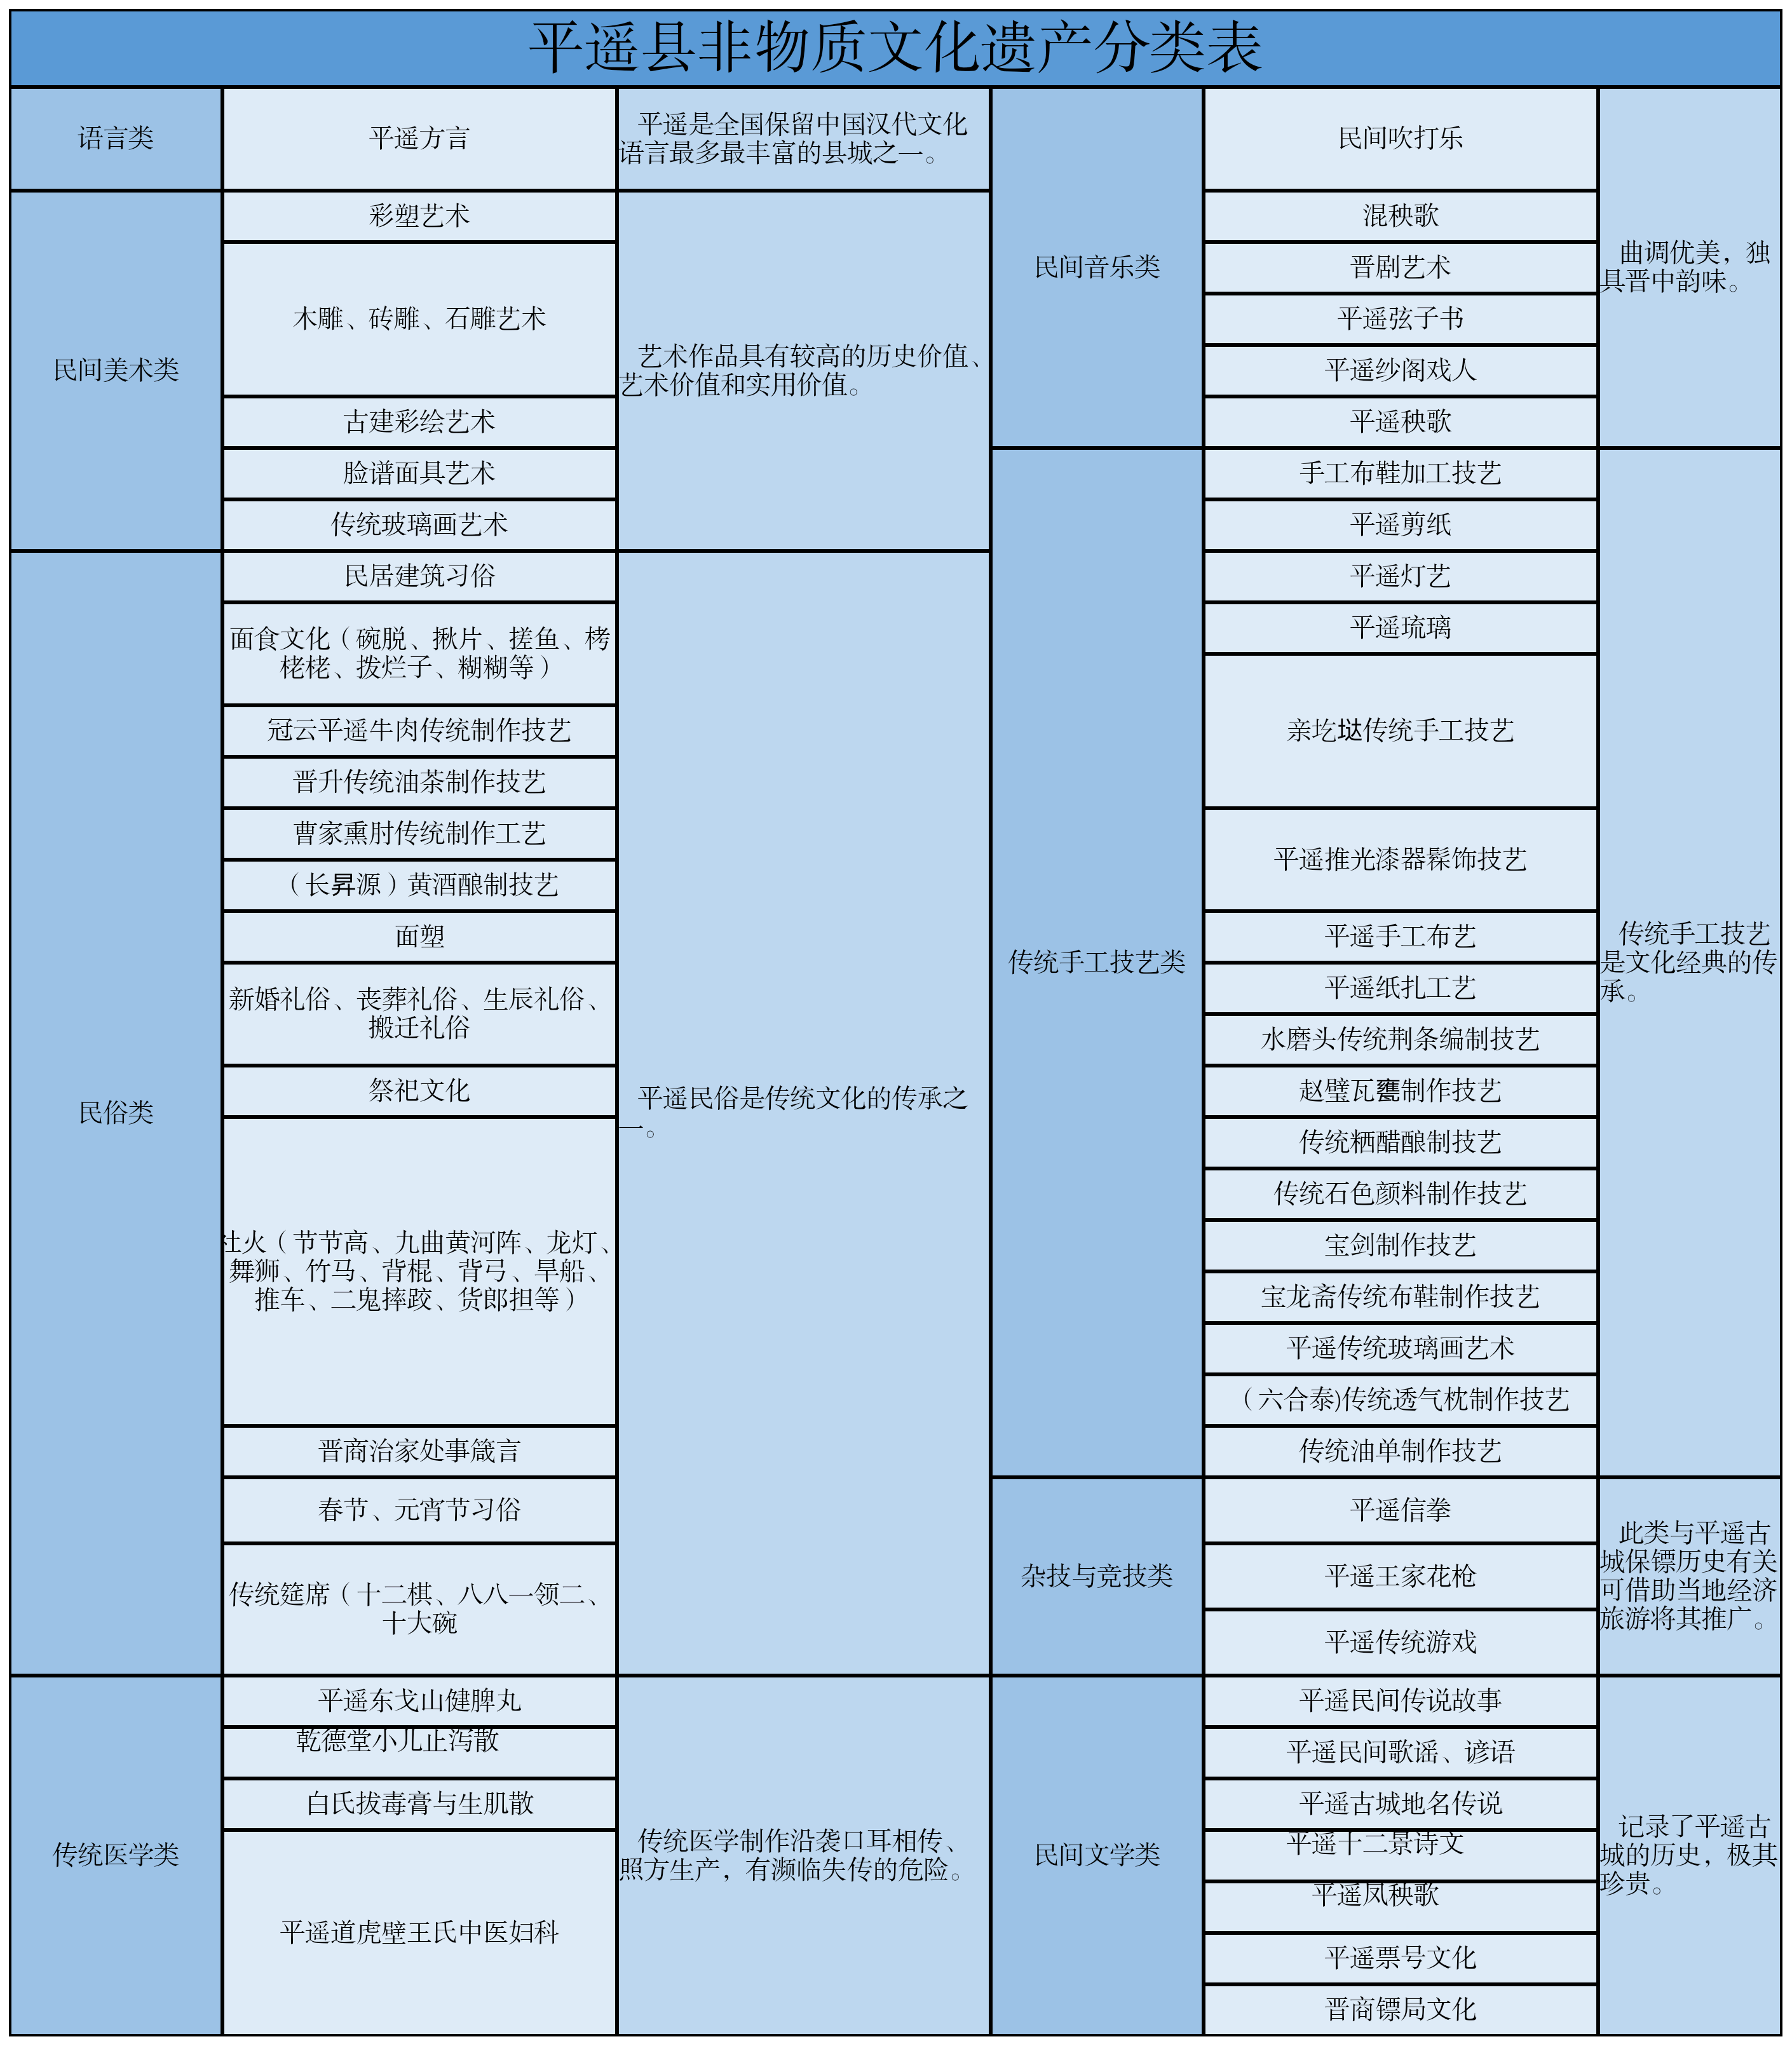
\includegraphics[width=7cm]{非物质文化遗产.png}
    \label{fig:my_label}
\end{figure}
\begin{figure}[H]
    \centering
    \caption{平遥物质文化遗产}
    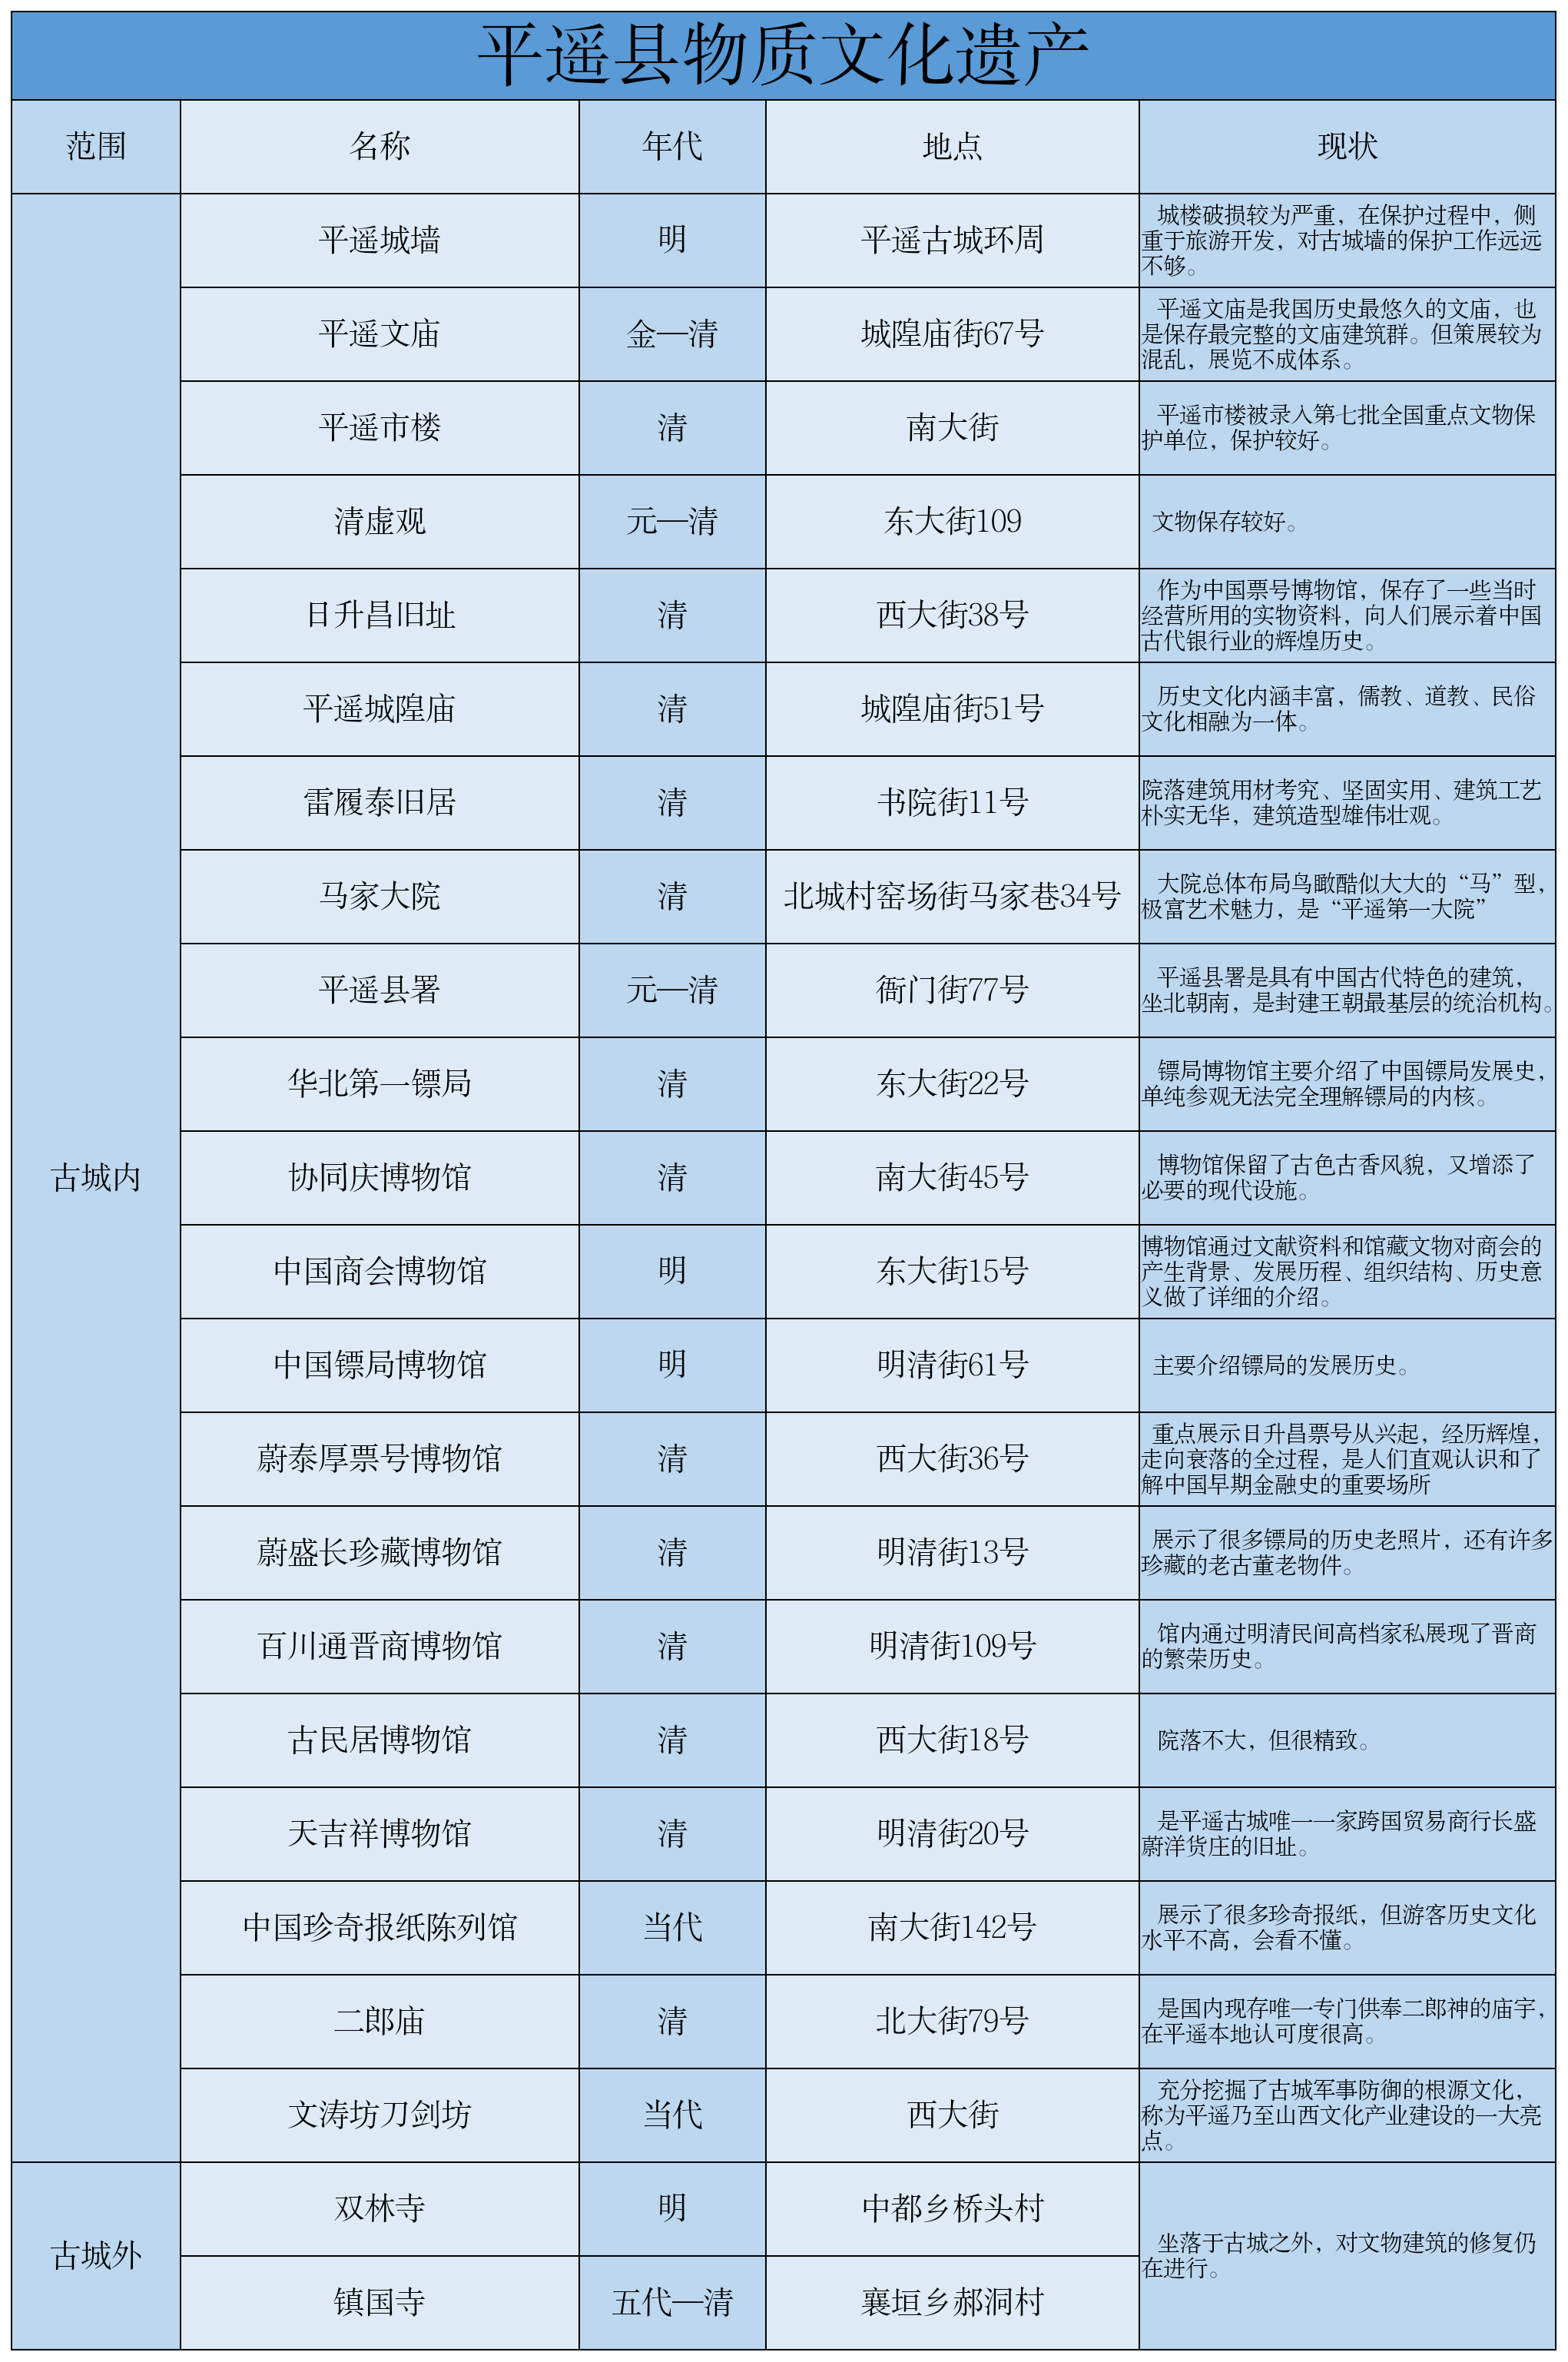
\includegraphics[width=7cm]{物质文化遗产.png}
    \label{fig:my_label}
\end{figure}
平遥县历史悠久,先贤给平遥留下了宝贵的物质财富和精神财富,既有古建筑古物品方面,又有很大的非物质文化印记。平遥县非物质文化遗产浩如烟海,种类繁多:不仅上可列入国家级省级,下至市级县级;又囊括语言,民间美术和民俗等各遗产种类。随着社会经济的发展,年轻群体越来越对非物质文化燃起了极大的兴趣和热情。基于此类市场群体的扩大和平遥文化遗产吸引力的增强。
    \subsection{平遥古城文化遗产保护与利用概况}
    1997年,平遥古城被列入世界文化遗产目录,与同为第二批国家历史文化名城的四川阆中、云南丽江、安徽歙县并称为“保存最为完好的四大古城”。

    近年,平遥古城以古城墙,古街道,古建筑的保护为前提,秉持着“保护为主,抢救第一,合理利用,加强管理”的发展理念,成功树立 了 以古城为核心的旅游景区 品 牌。据了解,全县形成了 以“一城两寺”24处景点、 6条特色街区(东、西、南、北大街,城隍庙街,衙门街) 、 3个演艺(又见平遥、晋商乡 音、迎宾仪式)为重点的旅游产品 体系,以文化资源为依托的文化旅游产业快速发展,平遥古城也成为全省乃至全国极具知名度的旅游胜地。目前,平遥古城内现有各级重点文物保护单位28处,其中国家级文保单位7处,市级文保单位2处,县级文保单位19处,文物古迹众多。除传统旅游资源外,现代节庆展览等文化旅游已成为平遥最具活力和最具发展潜力的朝阳产业。
    \begin{table}[H]
        \centering
        \caption{平遥古城部分节庆展览活动}
        \begin{tabular}{p{4cm}p{4cm}p{4cm}}
            \toprule
            节庆 & 举办年份 & 主题\\
            \midrule
            平遥国际雕塑节 & 2018第一届 &“中西方艺术文化交流”\\
            &2019第二届&“之间”\\
            &2020第三届&“生态美学”\\
            \cmidrule{1-3}
            平遥中国年&2018&“欢歌迎春”、“翰墨同春”、“彩灯靓春”、“社火闹春”、“民俗乐春”、“网络贺春”、“戏曲唱春”七个板块\\
            \cmidrule{1-3}
            平遥摄影大展&2016&“天地心·家国情”\\
            &2017&“回望初心·梦幻未来”\\
            &2019&“守正·创新”\\
            \bottomrule
        \end{tabular}
    \end{table}
    然而与此同时,在新冠疫情影响之下,病毒传播速度快,辐射地域广,对涉及人员流动的旅游业来说,影响也愈加广泛和深刻。在2020年初新冠疫情到来时,平遥古城自觉关闭所有商铺门店,所有的旅游从业人员暂离岗位,景区经济收入下滑严重。世界遗产平遥古城———如何在疫情的冲击下,发挥维持地方社会经济发展中的重要作用成为当务之急。如今正处于疫情防控后期阶段,景区采用了限制游客最大承载量、要求游客佩戴口罩、提供健康码以及保持1.5米间隔距离等通用安全防护措施,对古城旅游采用免门票的短期措施,以此来刺激旅游和经济的恢复。
    \begin{table}[H]
        \centering
        \caption{平遥古城游客接待量数据大致汇总(单位:万人次)}
        \begin{tabular}{p{2cm}p{2cm}p{2cm}p{2cm}p{2cm}p{2cm}}
            \toprule
            年份 & 国庆&清明&端午&春节&元旦\\ 
            \midrule
            2019& & & 11.52 & 45.39 & 1.6\\ 
            2018& 62.8 & 11.65 & 11.25 & 43.01 & 1.59 \\ 
            2017& 61.1 & 11.30 & & & \\ 
            \bottomrule
        \end{tabular}
    \end{table} 
\section{古城文化遗产保护和利用的分析}
    \subsection{平遥古城服务设施现状}
        \subsubsection{卫生设施}
        首先厕所的安排暂不合理,明清一条街上没有设立公共厕所,而在居民区和较为偏僻的小巷,公共厕所之间相差50米左右。此外,厕所的新旧程度不一,有些建设风格与古城整体不符,同时个别厕所内蹲位的设置以及卫生情况不太理想。
        \begin{figure}[H]
            \centering
            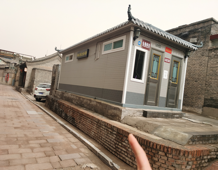
\includegraphics[width=6cm]{图片 1.png}
            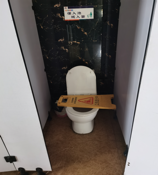
\includegraphics[width=4cm]{图片 3.png}
            \caption{平遥古城内的卫生设施\\料来源:团队摄于平遥古城内南大街}
            \label{fig:my_label}
        \end{figure}
        \subsubsection{道路设施}
        据考察发现,步行街一直存在不断修路铺路的工程。由于存在道路障碍,一些游客的绕道而行一定程度上减少了部分商铺的经营收入。另外,地面排水设施存在隐患,井盖之下,充满臭气的脏水位线过高,下雨之季积水上涨极大可能造成道路行驶不便。
        \subsubsection{交通设施}
        行街设置的多处栏杆,虽然直接避免了机动车的通行,但是也阻隔了婴儿推车、小型电动车、游览车以及自行车的正常进出,带来不便。此外,在停车场建设方面,北门和南门共有2个停车位,较为合理。但是古城内机动车的摆放仍要加强管理。
        \begin{figure}[H]
            \centering
            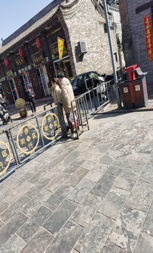
\includegraphics[width=4cm]{图片 10.png}
            \caption[plain]{栏杆\\资料来源:团队摄于平遥古城内南大街}
            \label{fig:my_label}
        \end{figure}
        \subsubsection{标识系统}
        过调查问卷得知,游客对古城内景点的游览图和指示牌满意程度不高,指示牌不够亮眼,存在数目不足的问题。
        \begin{figure}[H]
            \centering
            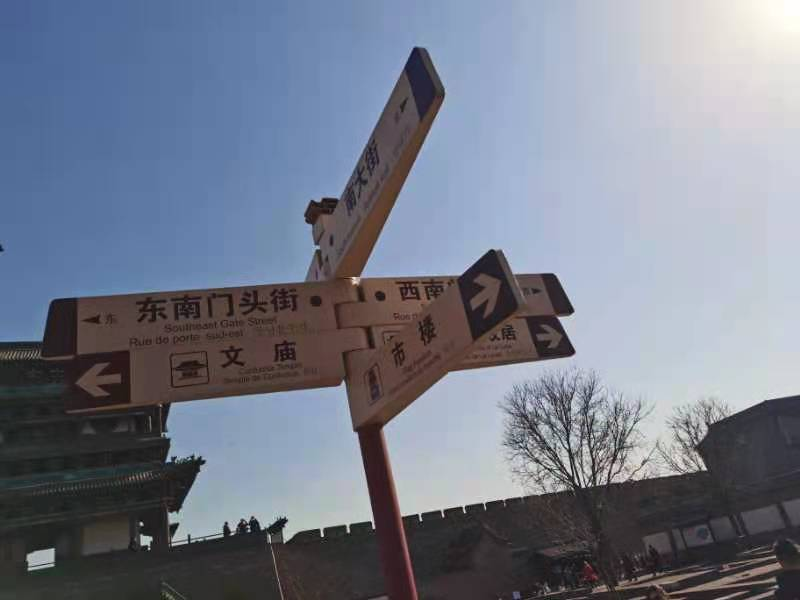
\includegraphics[width=8cm]{标识.jpg}
            \caption[plain]{平遥古城内的标识系统\\资料来源:团队在2021年3月摄于平遥古城南门}
            \label{fig:my_label}
        \end{figure}
        你看人家那个丽江古城、凤凰古城,灯火辉煌的多好看。本来工程量不大,现在动工的影响挺大的。
        
        \begin{flushright}
        ——砖雕店老板,2021年3月
        \end{flushright}

        \subsubsection{灯光设施}
        夜晚的古城,光源大部分来源于商铺,而用于道路照明的基础设施,明显不能够发挥作用,中心的市楼在晚上不被照亮,亮化设施存在开发潜力。
        \begin{figure}[H]
            \centering
            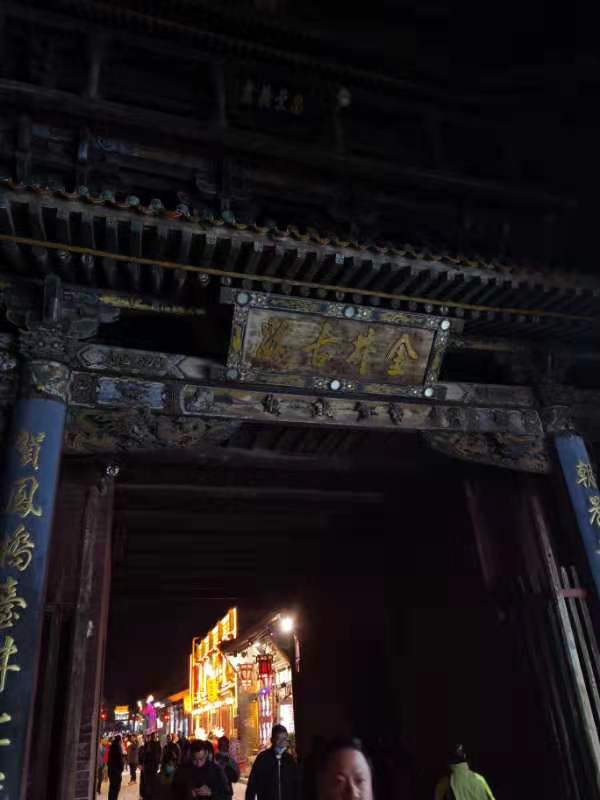
\includegraphics[width=6cm]{市楼亮化.jpg}
            \caption[plain]{晚上昏暗的市楼\\资料来源:团队在2021年3月摄于平遥古城南门}
            \label{fig:my_label}
        \end{figure}
        \subsubsection{消防设施}
        古城内放置的消防设备较少,只有城墙及部分景点有消防沙及水缸的放置。但是在居民区及古城街道等地方,消防设备放置较少且不规范。对木质建筑较多的古城存在较大威胁。
        \begin{figure}[H]
            \centering
            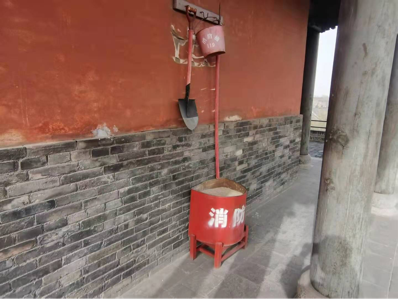
\includegraphics[width=7cm]{图片 15.png}
            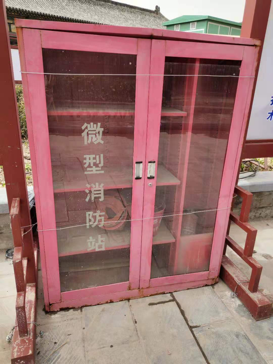
\includegraphics[width=4cm]{图片 17.png}
            \caption{消防设施}
            \label{fig:my_label}
        \end{figure}
        \subsubsection{环卫设施}
        古城内居民垃圾分类意识不强,没有关于垃圾分类的规章制度。而乱七八糟的垃圾随意混杂在一起会对其他可回收利用的垃圾造成二次污染,导致可回收利用的垃圾不可再回收,使得资源浪费。
    \subsection{平遥古城文化载体保护利用现状}
    古城内的大部分建筑都为砖、木制结构,大部分古建筑都有不同程度的破损。建筑主体的破损直接影响到古建筑的完整性和游客的体验感。景点内的水缸有掉漆现象,双林寺的大门也比较破败,直接影响到游客对景区的第一印象。
    \begin{figure}[H]
    \centering
    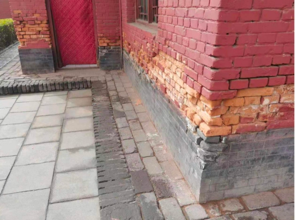
\includegraphics[width=4cm]{图片 19.png}
    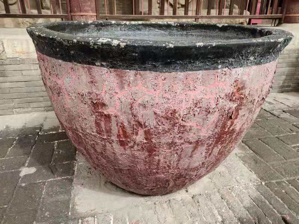
\includegraphics[width=4cm]{图片 20.png}
    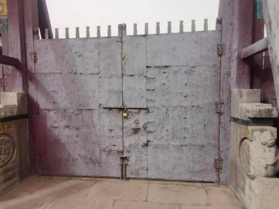
\includegraphics[width=4cm]{图片 21.png}
    \caption{古建筑}
    \label{fig:my_label}
    \end{figure}
    古城内城墙破损现象比较明显,北门和南门附近的城墙都有较严重的破损。城墙损坏严重,采用的填土护坡方法,这种方法采用在古城墙一侧堆砌土方,用于加固原有城墙使之免受自然力侵蚀,此种方法虽然可以最大程度上还原古城面貌,但是防护效果较差,动用土方较多,且在后期维护时难以划清界线,为今后的养护工作带来不便。且相较用石头堆砌, 土方结构较为危险。
    \begin{figure}[H]
    \centering
    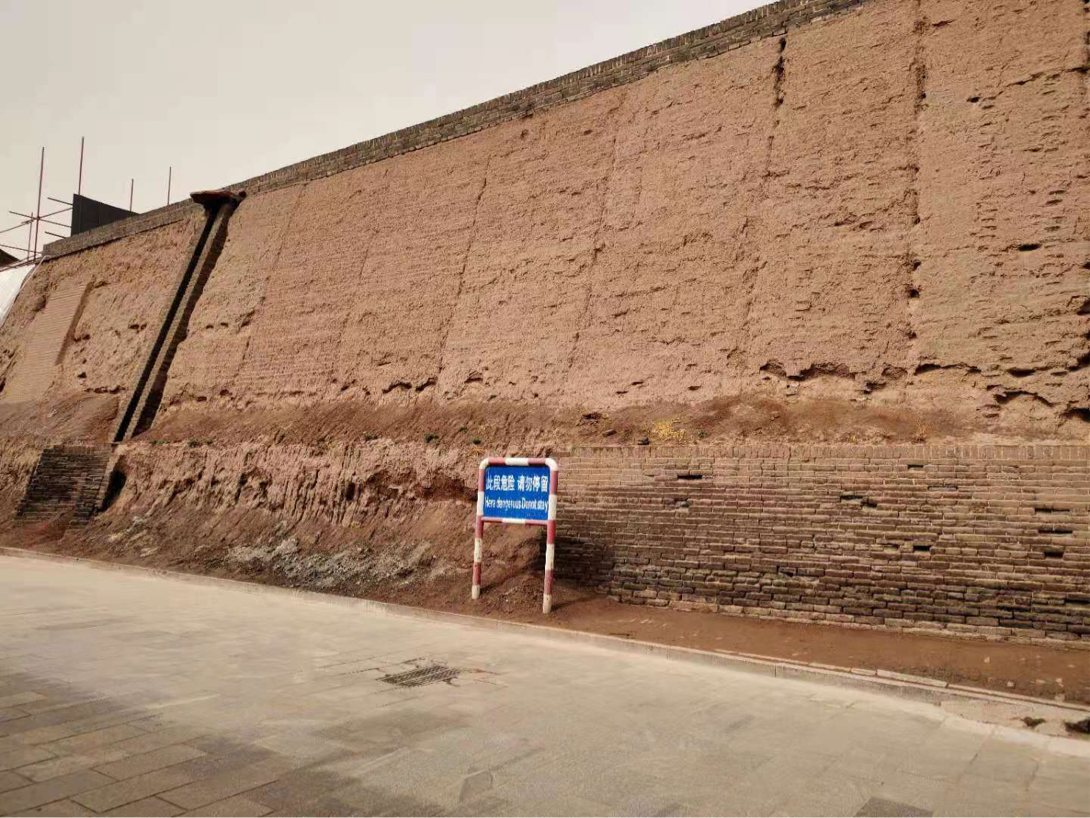
\includegraphics[width=5cm]{图片 23.png}
    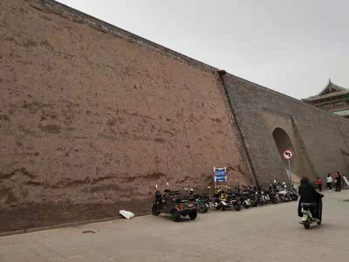
\includegraphics[width=5cm]{图片 24.png}
    \caption{破损的城墙}
    \label{fig:my_label}
    \end{figure}
    \subsection{平遥古城非物质文化遗产保护利用现状}
    我们这个面馆还是有一些老顾客的,让顾客写下这些便利贴,有对我们的建议与自己的心愿。我们是想通过这个监督自己,更好的满足顾客的需要。

    \begin{flushright}
        ——北门老刘家罐罐面店主老板娘,2021年3月
    \end{flushright}
    
    从北京回来以后,我们更多的是想在家乡发展,平遥古城以晋商文化闻名世界,我们想把自己家乡的这种文化传承下去。经营的过程中,利益肯定是一方面要考虑的因素,当然我们更多的是要为顾客考虑,不能单纯的是为了盈利,主要是有这个情怀在里面。
    \begin{flushright}
        ——洪武记饭店青年创业者老板,2021年3月
    \end{flushright}
    \hspace*{\fill}
    
    继承是发展的前提,发展是继承的必然要求。
    
    垂暮蔼蔼,引水活源。对世界文化遗产的保护不仅要让故有之姿恢复原貌,同时也要将古城融入现代社会的潮流中。原封不动的维护只会淡化这座历史遗迹的“烟火气”。要让古城洗尽尘埃,带着历史的气息贴近群众,必然要把旅游业作为古城保护与发展的重要战略。
    
    随着近年来文化遗产旅游(cultural heritage tourism)的悄然兴起,游客对旅游地附加体验的要求越来越高。平遥古城在此基础上所具备的主观条件便是丰富的非物质文化遗产, 在过去几十年的发展中,古色古香的建筑城楼无疑成为平遥古城一张亮丽的名片,古城也 以极大保留明清时期县城的基本风貌这个突出特点为旅游发展喊出“历史感”的口号,但在实际发展的过程中,蕴含在古城中的非物质文化遗产在一定程度上并没有得到很好的展现。        \subsubsection{民俗传承}
        平遥古城不但浓缩了历史的古朴厚重,同时也承载着绵延不绝的生活气息。平遥民俗是传统文化的传承之一,反映了一代代人对生活的热爱,是一个地方生活气和烟火气的集中体现。结合资料和实地考察发现、节节高、九曲黄河阵、背棍、舞狮、旱船、二鬼摔跤以及货郎担等民俗类文化遗产在平日里较为少见,只作为一些节日里的特殊产品,宣传措施环节也较为薄弱,相当一部分游客表示对它们并不了解。而在面塑、黄酒油茶等传统制作技艺的传承上,也大多停留在商铺推出的一些假人泥塑表演层面。而平遥秧歌、弦子书、纱阁戏人以及平遥琉璃等种类繁多的民间音乐类文化遗产,也在平遥人们的生活中被束之高阁。由此可见,平遥民俗众多,但是宣传和推广力度不足以让其吸引游客,扩大市场范围。      
        \begin{figure}[H]
            \centering
            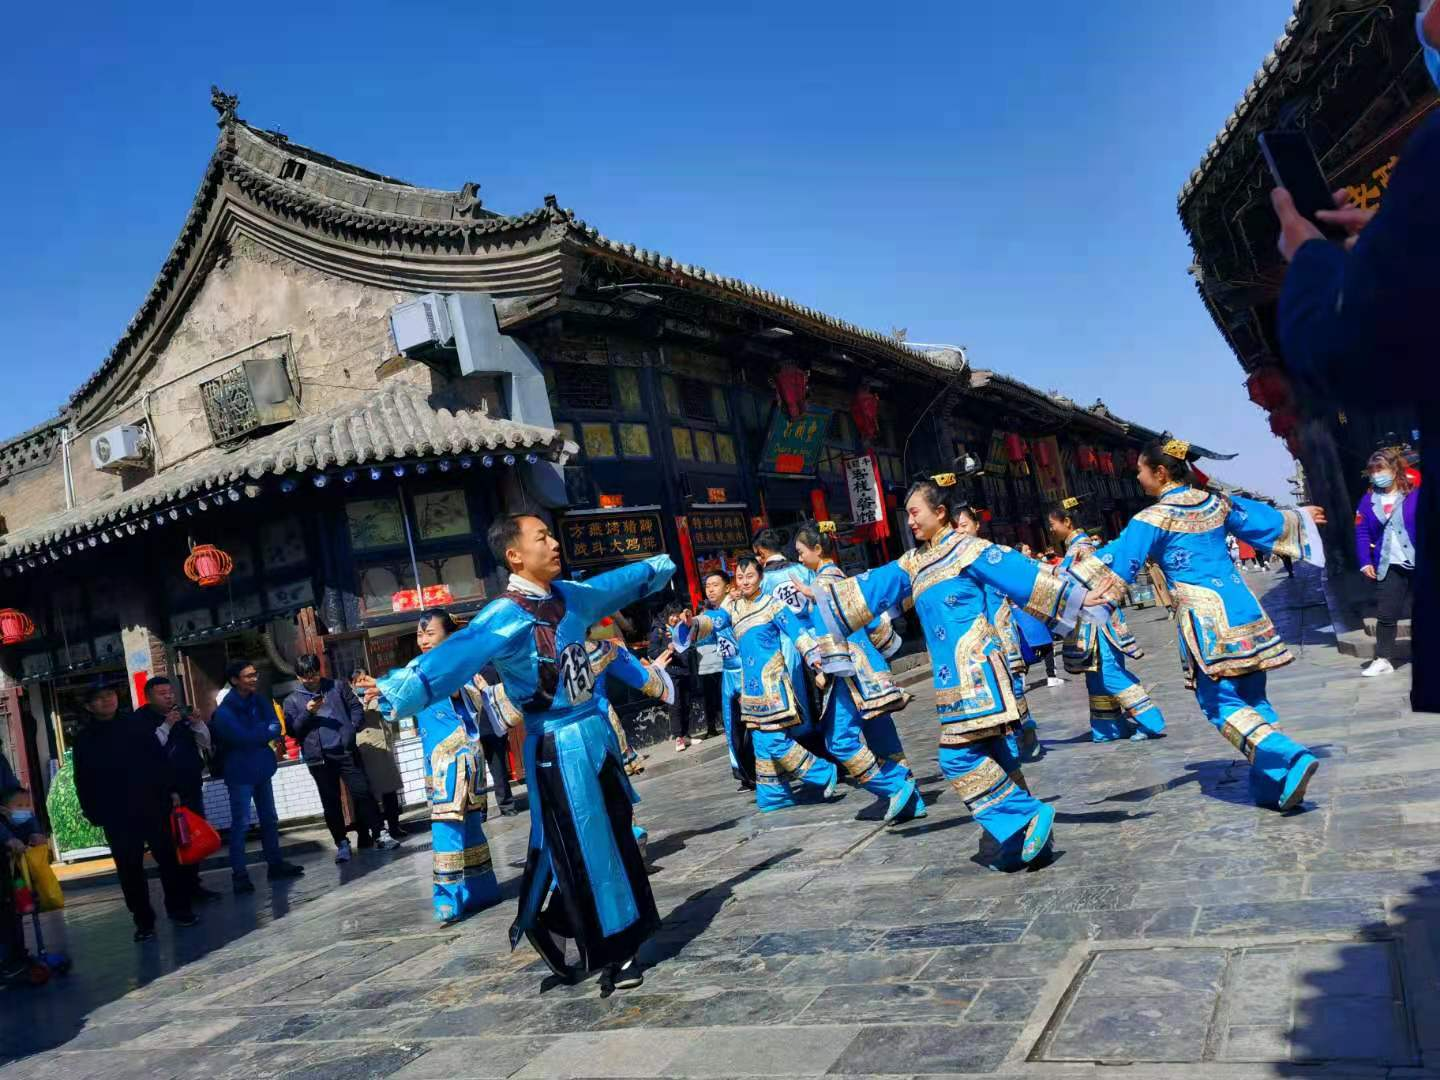
\includegraphics[width=7cm]{表演.jpg}
            \caption[plain]{平遥古城内的文化表演\\来源:团队摄于平遥古城南大街街口}
            \label{fig:my_label}
        \end{figure}
        \subsubsection{品牌内涵}
        有一个奶茶店前年还是去年开的,也学我们,但后来还不是开不下去,今年关了。
        
        \begin{flushright}
            ——在梁先森の酸奶铺子工作的店员,2021年3月
        \end{flushright}   
        
        近年来,古城内产品同质化现象严重,商铺所销售的商品仅以产品命名,缺乏个体鲜明的独特标识,品牌建设意识不强,这些导致游客对百年老店和非官方门店的辨识度不高。在平遥古城内的商铺竞争中,仍然存在抢占客源恶性竞争的问题,多家出售醋酒的门店经营时间不尽相同,但装修风格和产品种类大体一致,这让初来的游客无法辨认选择真正认可的产品。借此对比,2021年新推出的“又见平遥精酿啤酒”概念装设计以新颖独特的设计,获得了意大利a design word \& competition青铜奖,其他品牌建设则可以以其为灵感依托,开发更多品牌,促进改善竞争环境,繁荣新兴市场,最终为游客营造舒适的游客体验。
        \subsubsection{晋商文化}
        北京回来以后,我们更多的是想在家乡发展,平遥古城以晋商文化闻名世界,我们想把自己家乡的这种文化传承下去。经营的过程中,利益肯定是一方面要考虑的因素,当然我们更多的是要为顾客考虑,不能单纯的是为了盈利,主要是有这个情怀在里面,尤其是在疫情期间。
        
        \begin{flushright}
            ——洪武记饭店青年创业老板,2021年3月
        \end{flushright}

        在疫情的冲击下,大多数商铺响应国家地方政策全部关闭,店主和员工也因失去了唯一的经济来源而陷入困境。因此,如何传承以“进取、敬业、群体”为核心的晋商精神、增强经济的抗压度和韧性也成为了一个亟待深思的问题。另一方面,从旅游体验角度上看,商铺本身承载的晋商文化在营造良好商业氛围的同时,为游客创造了独特的旅游体验,形成一个真正的“情怀氛围感染圈”,吸引更多的游客前来体验,增加晋商文化与古城融为一体的印象。
        \subsubsection{风土人情}
        纵观商业集中地区——明清一条街,各种类型的商铺都有存在,平遥古城特色商铺混杂经营于众多商店中,明清古街更像是普通的商贸区。古城内与古城外售卖种类相差无几。
    
        另外户籍居民中的部分群体在非户籍人口进城经商挤占市场份额的冲击下迁往外城,原生居民也带走一部分古城本土文化的气息。2020 年新冠疫情加速了这一进程,随着古城整顿与修复的进程,本地居民的收入水平也不足以支持原有生活。外来居民在一定程度也冲淡了本土文化。
        \begin{figure}[H]
            \centering
            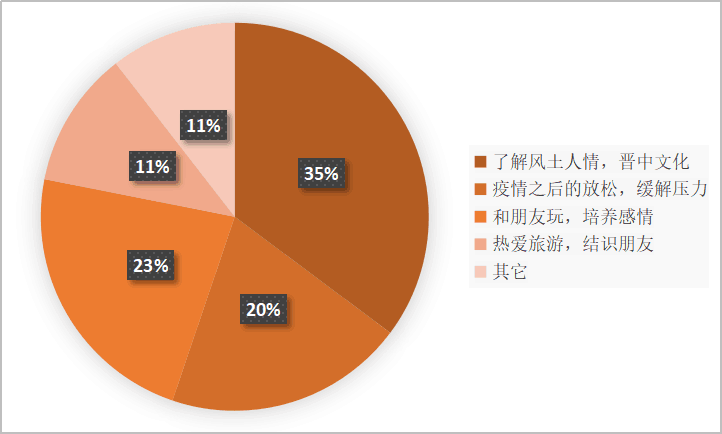
\includegraphics[width=8cm]{游客目的.png}
            \caption{游客目的饼图}
            \label{fig:my_label}
        \end{figure}

        古城悠久的人文历史确实可以吸引四方游客来此地进行一场“古今对话”的旅行,但是要以此作为旅游业发展的全部基点是远远不够的。短暂的接受历史知识、接触独特的晋商文化无法让游客真正体验到一次平遥古城之行的乐趣。必须从多个反面考虑,结合“个性旅游”、“定制旅游”的新趋势,基于古城自身的特色,为游客的旅程增添新的涵义与内容。

        从旅游的六大因素——“吃、住、行、游、购、娱”分析,游客在古城的最大消费主要集中在饭店、酒店、商铺以及娱乐性活动的参与。为了能让游客在旅行的过程中留下深刻印象,毫无疑问要把平遥古城传统的、个性的方面挖掘出来,将平遥本地特色与游客集中点联系起来,以游客需求为导向,变作古城的一种内在特征。

        \subsubsection{文化产品}
        我觉得这里有本地特色的纪念品太少了,和别的旅游地方没什么区别,卖的都是一样没有新意。我们现在出来玩,就是想看些特色的玩意儿,像刺绣啊编织框啊,我们就好这一口,可以买来做纪念,摆放在家里。
        
        \begin{flushright}
            ——中年女游客,2021年3月
        \end{flushright}

        古城内一些文创商店所售皆为日常生活所见的物品,稍加一些古风、古玩的特点,且物价高,导致不仅销售量极低,同时无法满足游客需求。平遥古城传统手工技艺闻名世界,许多慕名前来的游客见到的更多的是老店——推光漆器、老陈醋、平遥牛肉等。尽管价格对不同的群体反响不同,但是产品种类少、价值不副其实是游客共同的反映。
    \begin{figure}[H]
        \centering
        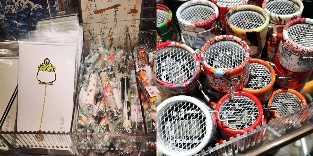
\includegraphics[width=8cm]{文创1.jpeg}
        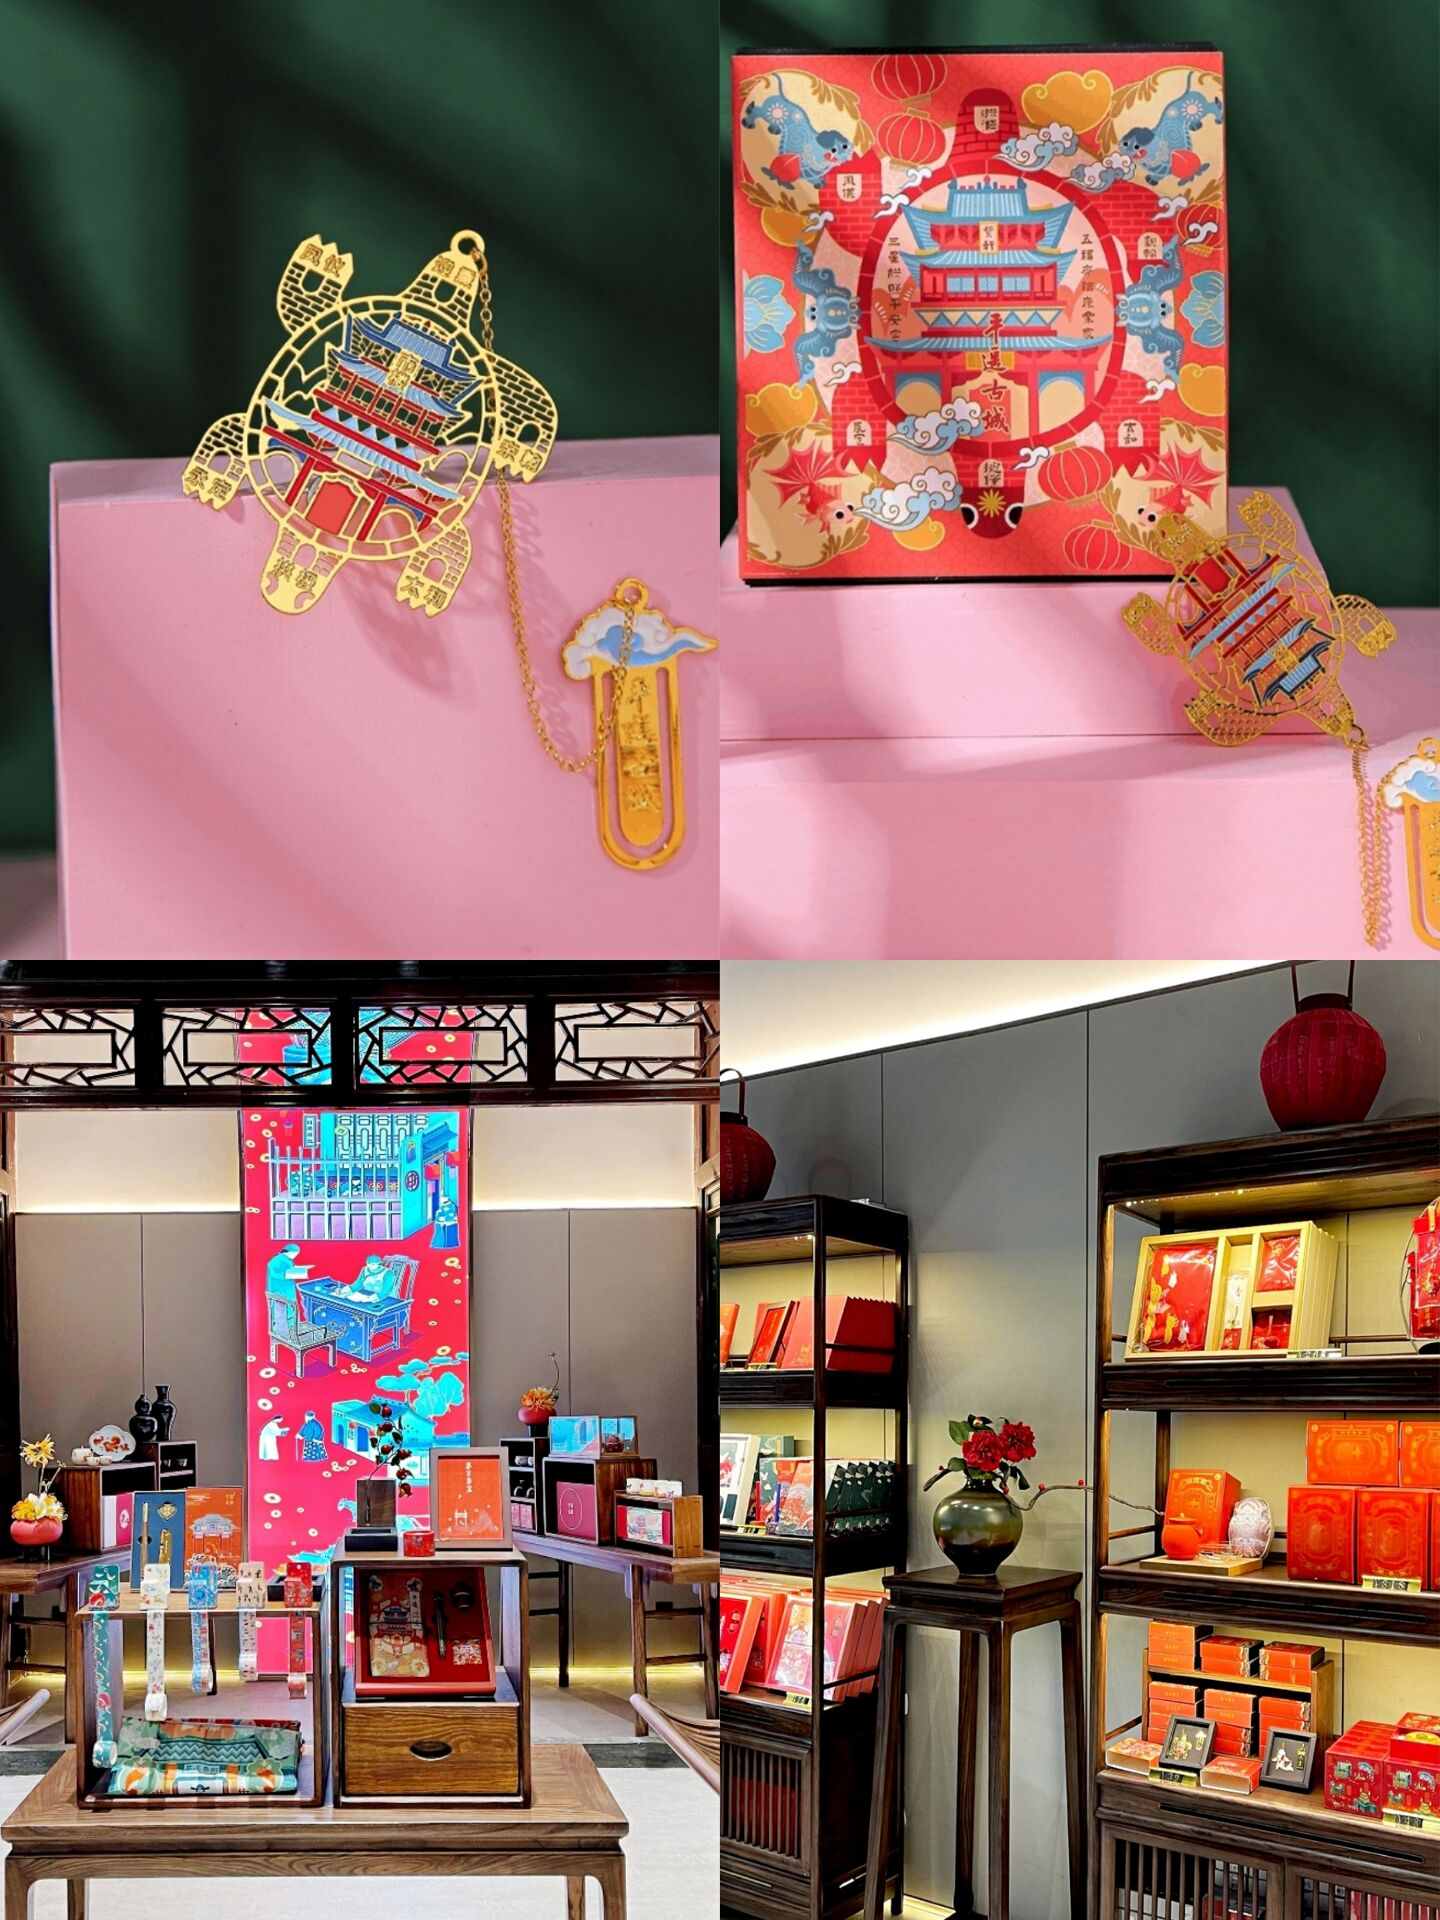
\includegraphics[width=3cm]{文创拼图.jpg}
        \caption[plain]{截止2021年3月 左图为平遥古城内最常见的文创产品,右图为平遥古城最新文创产品\\资料来源:团队在2021年3月摄于平遥古城内文创店(左一、二)\\右一来源于平遥古城景区官方服务平台公众号}
        \label{fig:my_label}
    \end{figure}
    同时,产品同质化严重,导致游客对官方与非官方产品的辨识度不高,消费环境安全系数低。商铺所售商品仅以产品命名,缺少品牌意识。
    \\\hspace{\fill}\\
    
    (疫情)以前还有些游客,现在几乎没有人了,就是凑合的过日子,收入就没有来源了。
    
    \begin{flushright}
        ——五则副食店老板娘,2021年3月
    \end{flushright}
    
    古城交通管控的比较严,我们这样的三轮车进不去,人家大门店也不招我们这些人,想挣点小买卖也得辛苦点出去走街串巷。
    
    \begin{flushright}
        ——在北门和西城村贩卖糖葫芦的街头商人老奶奶,2021年3月
    \end{flushright}
    
    (对自己的生活)非常满意。国家不管农民还是市民都是补贴 123 块,全县统一的。
    
    \begin{flushright}
        ——街边闲坐的大爷,2021年3月
    \end{flushright}
    
    不行,不够活,你们看我这衣服——穿了好几年了。我们出来没有买过古城里的东西,也不知道贵不贵。封城的时候,是我们家亲戚给我们捎进来一些蔬菜。
    
    \begin{flushright}
        ——西城村老奶奶(市民),2021年3月
    \end{flushright}
    
     
    \subsection{平遥古城景区综合治理现状}
    从实地采访的结果来看,政府在发展平遥古城的经济的过程中,实施了诸多有效措施, 基本改变了古城贫穷落后的面貌,居民的幸福感指数大幅度上涨。但是随着旅游业的发展, 其自身暴露的许多问题也同样充斥着居民的生活,从另一方面给古城发展带来不利影响。

        \subsubsection{居民区风貌落后,发展水平较低}
        \begin{figure}[H]
        \centering
        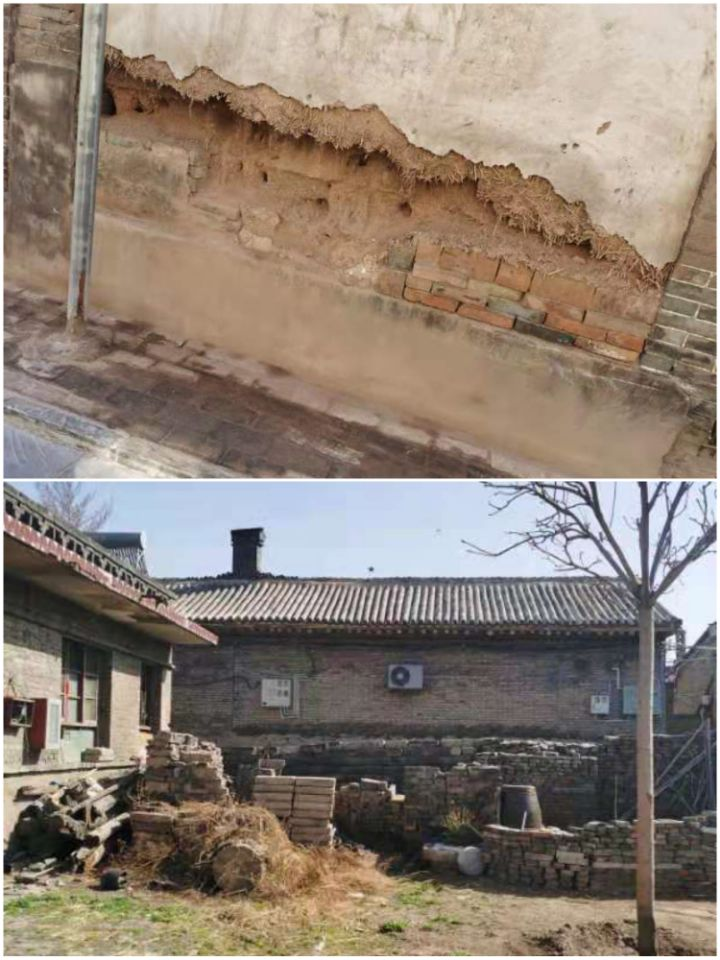
\includegraphics[width=6cm]{建筑.jpg}
        \caption[plain]{平遥古城内的旧建筑\\资料来源:团队在2021年3月摄于平遥古城西城村}
        \label{fig:my_label}
        \end{figure}
        旅游业的发展一定程度上拉大了居民贫富差距,新冠疫情的爆发使这一问题彻底暴露出来。居民区出“空房无人”的情况,部分居民生活困难,相对封闭的环境导致思想趋于保守,居民区逐渐“空心村化”。
        
        由于完整的文物古迹多数位于古城南部,北部游客量极大程度上少于南部。客流量的不平衡导致了南北租金差距大,加上北部大面积为原始村落,属于本地居民生活区,古城北部的发展明显不如南部。
        
        此外,由于土地征收,部分农民转农从商,同时由于文化水平不高,只能从事一些服务型产业,或者租用个人门店从事小型商业,经济收入依附于旅游业,极具脆弱性,因此遭受疫情的冲击影响较大。窘迫的经济环境迫使年轻劳动群体虽然仍从事古城旅游业,但选择离开古城生活。对于一些行动不便,缺乏知识的老年群体只能依靠国家补助维持生活。
        
        再者,平遥古城属于世界级文化遗产,客源地不乏为经济水平极高的区域。平遥古城所展现出的落后农村气息会在视觉感官上影响游客旅行体验。有必要改变整体村落风貌,进一步改善居民生活水平。
        
        \subsubsection{旅游业体系单一,呈畸形发展趋势}
        
        随着古城旅游业的发展以及旅游市场的进一步开放,市场经济的盲目性也日益凸显,诸多人员投入到服务行业,导致旅游业所提供的服务质量参差不齐,甚至影响到游客利益。“黑店”、“宰客”的不良现象不断发生,欺诈型消费直接导致游客对古城的印象与满意程度下降,继而影响古城旅游业的整体发展。
        
        另一方面,古城旅游业主要依靠门票来拉动。官方价格为125元的古城通票,虽然包含22个景点,但是普遍受到游客和商铺的非议。平遥古城“门票经济”特征突出。
        
        此外,古城占地面积 2.25 平方千米,城内街道错综复杂,导游与游览车服务占据重要作用,成为游客游玩必不可少的部分。从事此行业的人群众多,有当地旅行社集中管理的专业导游,也有本地居民为谋生借助自身的熟悉度为游客导路,比较特殊的是义务导游。这类导游分为两类群体,一部分是当地小学组织的学生义务讲解,这类群体虽然专业化水平低, 经验欠缺,但是深受游客喜爱,受众度比较高。另一部分是政府管理的旅游景点,委派专门员工负责为到访游客进行讲解,但是此类景区多是知名度较低,并且雇佣的员工也大多为非户籍群体。从种类上说,导游行业讲解人员各具特色,可以带给游客不同的体验。但是从数量上说,义务导游最为少见,居民导游次之。而占比比较大的旅行社导游与游客接触最多,管理问题也最大。根据实地考察发现,导游带团会到与旅行社有合作关系的固定商铺,这对一些中小型商铺的影响比较大,间接导致客源减少。使得商铺行业呈依托资产发展的体系,游客也从客观上无法接触更多的商品。
        
        由于旅游业所推产品种类较少,即文化创意产品、特色活动少,古城旅游业收入来源单一。政府要维持古城维修与保护的费用,只能依附于门票价格。然而,从数据分析来看,游客停留时间多为短期,并且个性爱好不同,“打包式门票”颇有些强制消费的意味。
        
        \subsubsection{防控意识不高,古城内外标准差别大}
        疫情期间,受封城的影响,居民物资补助困难,行政管理松懈。有一重要实例是,平遥古城景区管理有限公司于 2021 年 2 月 24 日下发文件《关于平遥古城景区调整疫情防控措施、3D 灯光秀恢复演出通告》,但在三月末景区入口处的防疫设施已经停用,工作人员对进城游客的检查较为松弛。见图
        \begin{figure}[H]
        \centering
        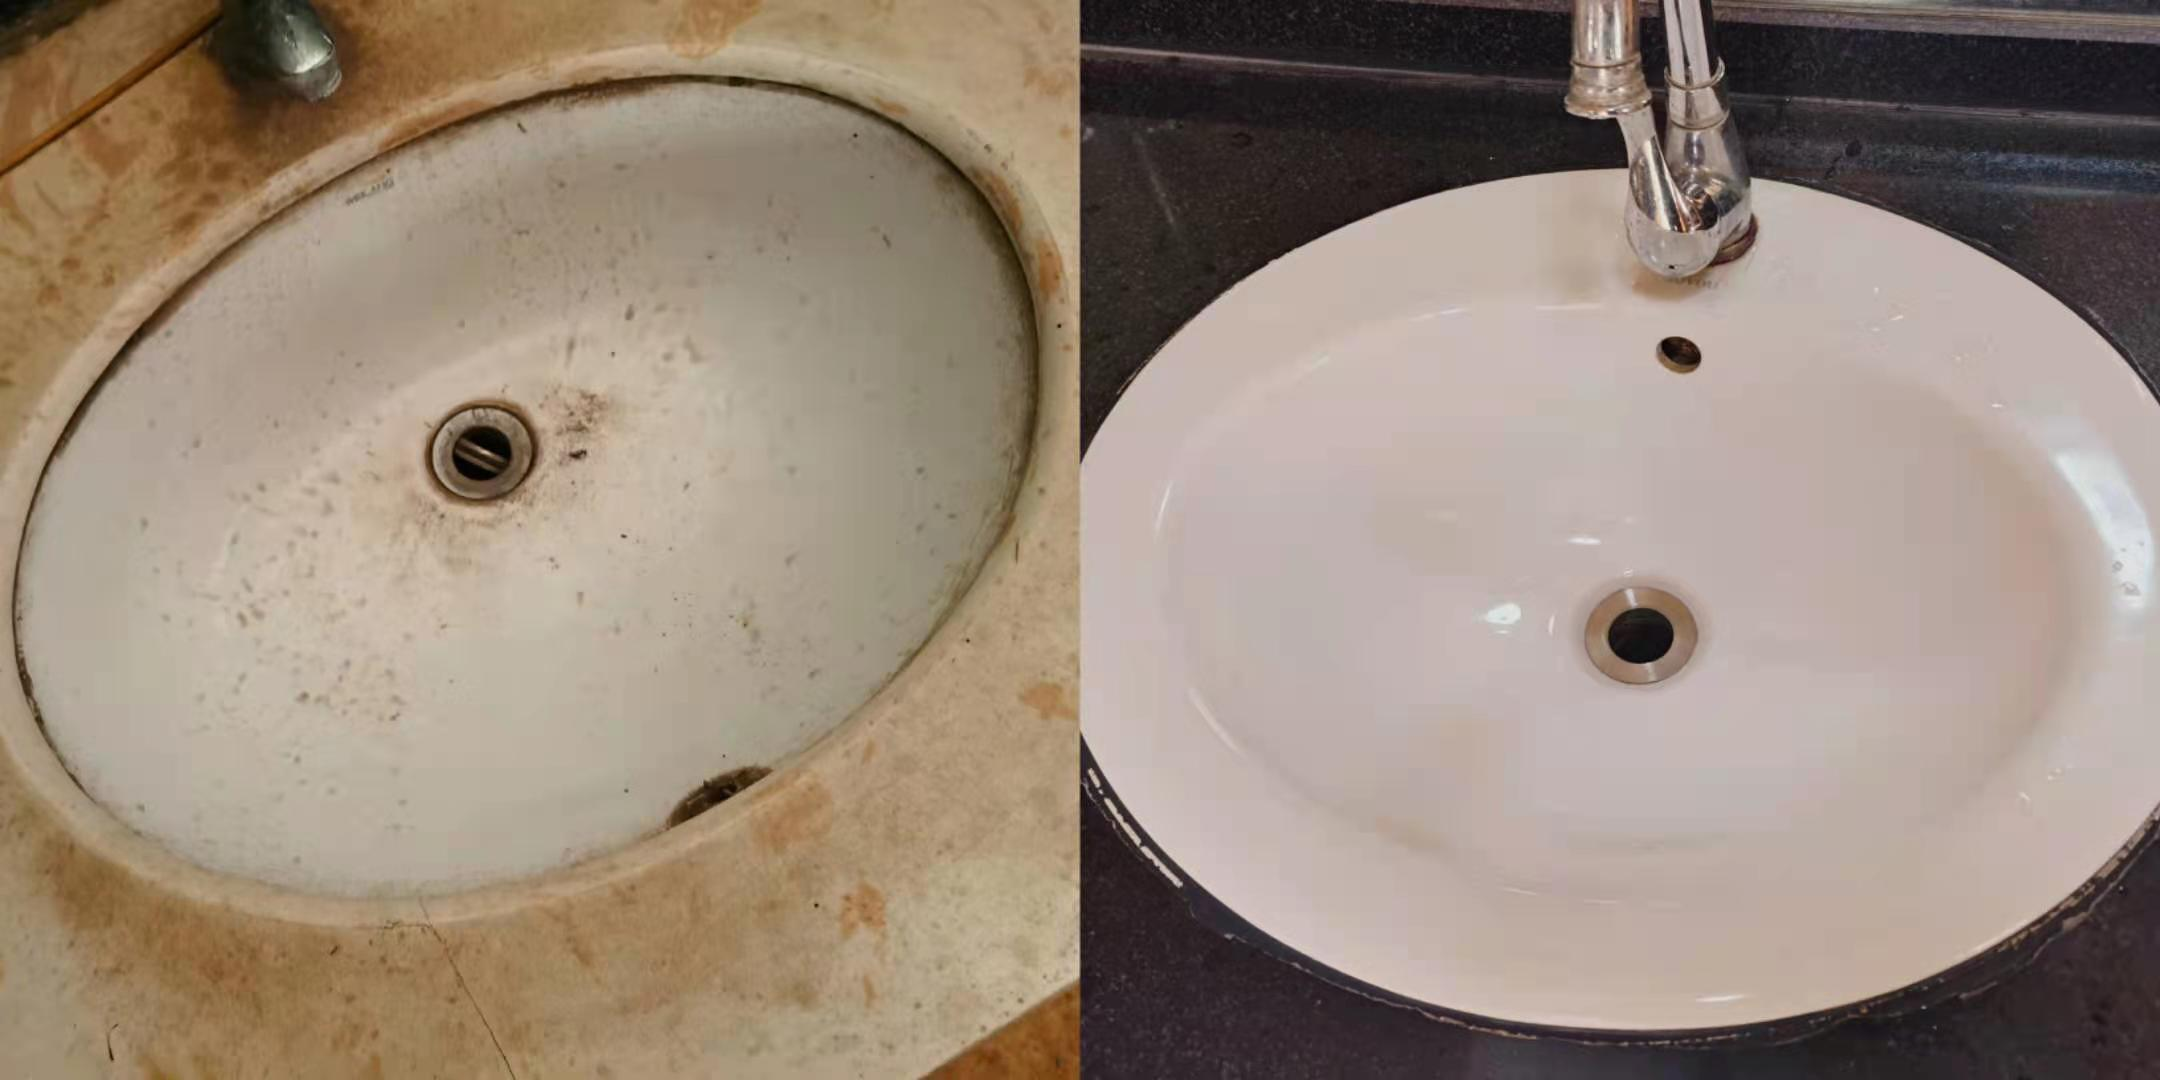
\includegraphics[width=7cm]{洗脸盆.jpg}
        \caption[plain]{公共卫生间的台盆\\资料来源:2021年3月左图于古城外摄,右于古城内摄}
        \label{fig:my_label}
        \end{figure}
        同时,古城内外卫生标准不统一,在平遥古城外围区,公共基础设施维护弱于城内。过渡区发展滞后,城墙内外景象对比强烈。
        
        一方面是古城受旅游业的影响飞速发展,商业经济不断扩大,另一方面是政府的政策与建设步伐较慢,与时代和发展的协同性低。
        \subsubsection{景点规划协同性差,旅游路线联通性低}
        \begin{figure}[H]
        \centering
        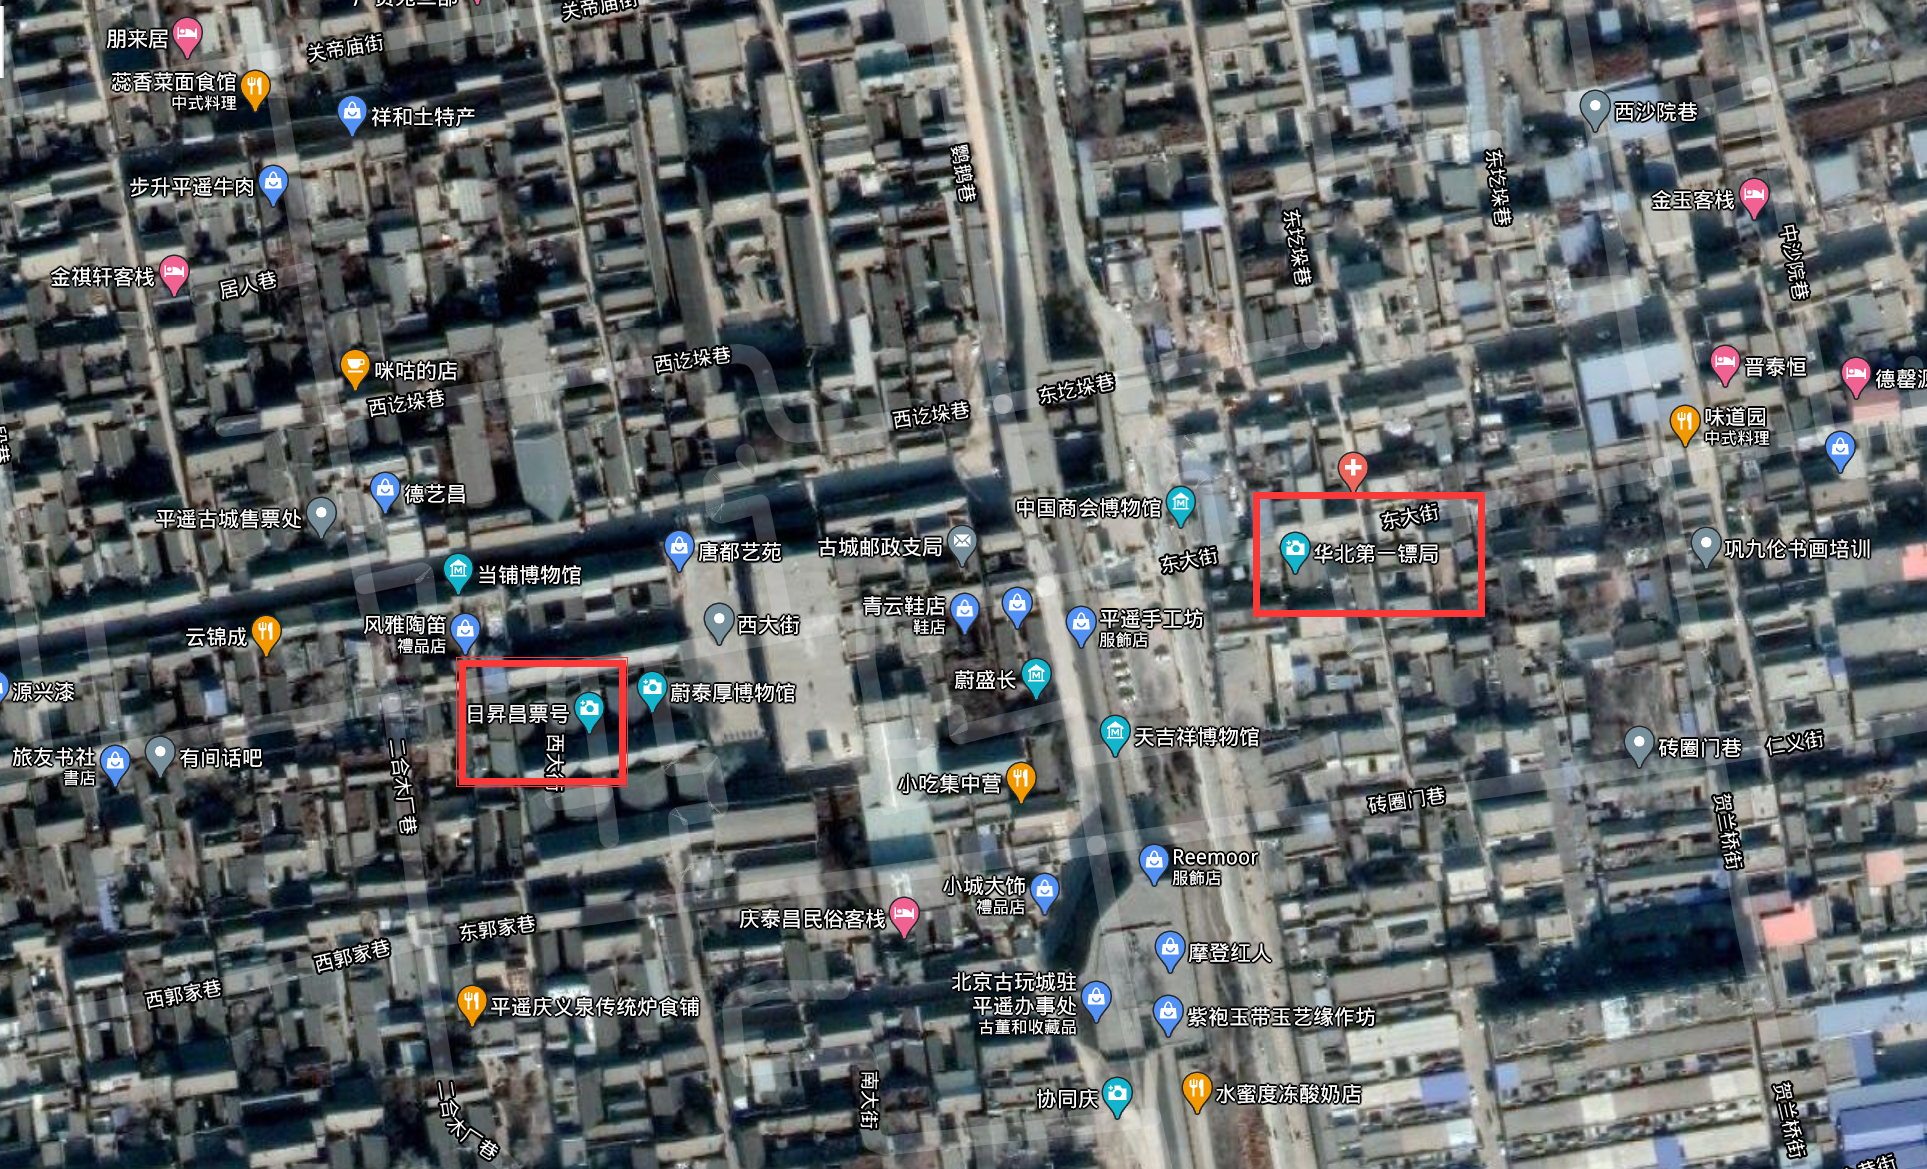
\includegraphics[width=7cm]{地图.png}
        \caption[plain]{平遥古城鸟瞰图\\资料来源:Google地图}
        \label{fig:my_label}
        \end{figure}
        平遥古城的景点较为分散,城外著名景点——双林寺和镇国寺分别距离古城南门 8 公里、15 公里左右,且在古城东西分布局,与火车站、高铁站距离同样很远,对于占比较大的一日游游客来说,分散的景点很难形成一个有效的旅游方案,在辗转的路上消耗就极大。对于古城内的景点同样如此,大部分景点东西对称分布,而景点之间的线路存在单一、游览价值低的情况,例如要游览日昇昌旧址与华北第一镖局博物馆就要将西大街来回走两遍, 倘若要观看有定点时间表演的景点,路程更是冗长。
        
        景点的分散造成了古城周围的空白区较多,也许一些地方在游客游览的过程中会经过, 但是缺少相应的游览点,游客的消费只能集中在来往的路途上。因此,鉴于游客量在不同地方的出入,政府对不同地方的管理程度也就不尽相同。
        
\section{平遥古城非物质文化遗产游客体验评价}
    \subsection{问卷设计}
        \subsubsection{问卷设计的思路及流程}
        在问卷设计上,我们将问卷分为三个部分,第一部分是游客的基本特征,包括性别、年龄、受教育程度和籍贯(客源地);第二部分是游客的活动特征,包括出游方式、旅游目的、游客停留天数、住宿选择、购物体验和古装意愿;第三部分要求游客采取五点量表\footnote{五点量表的评语等级分为非常满意、满意、一般、不满意、非常不满意等 5个等级。}法进行打分。分别是1-5分,在用综合评价法考察游客的主观感受时, 选取景观完整度、真实性、建筑、风土人情、特色住宿、特色餐饮、导游服务、标识系统、卫生整洁程度、交通便利程度、商业化程度、购物品12个指标,构成评价指标集。
        \subsubsection{指标权重的确定}
        在问卷中,对游客体验最为重要的莫过于第三部分的评价指标,故我们要对其进行综合评价,这里采用的是熵权法(Entropy Weight Method),这里的熵指香农(Shannon)的信息熵理论(Information Entropy Theory)\upcite{shannon1948mathematical},按照熵的思想,人们在决策中获得信息的多少和质量是决策的精度和可靠性大小的决定因素之一。计算出的熵权可以作为属性权重,熵权越大,权重越大,对应指标属性就越重要\upcite{农村老年人社区养老满意度及影响因素研究}。鉴于原始矩阵的篇幅,我们不能在此列出,于是我们只叙述计算过程。

        在原始矩阵$x_{ij}$中每一列为一个指标,每一行为每一个调查问卷中的分数,于是这个矩阵是$m \times n$的,在我们的例子当中$n=220$,$m=12$我们首先进行标准化处理,利用正向指标
        \[Y_{ij}=\frac{x_{ij}-\min\{x_{1j},...,x_{nj}\}}{\max\{x_{1j},...,x_{nj}\}-\min\{x_{1j},...,x_{nj}\}}\]
        其中$Y_{ij}$称为标准矩阵,在标准矩阵的计算当中,我们需要剔除评分单一的问卷,因为评价单一会造成
        \[\max\{x_{1j},...,x_{nj}\}-\min\{x_{1j},...,x_{nj}\}=0\]
        即除数为0的情形,而评价单一的问卷参考意义不大,故此处直接剔除,剔除之后的$n'=130$。接下来计算第$j$个问卷在第$i$个指标下的比重
        \[p_{ij}=\frac{Y_{ij}}{\sum\limits_{i=1}^{n'} Y_{ij}}\]
        我们得到的是概率矩阵,接下来只要通过
        \[E_j=-k\sum\limits_{i=1}^{n'}p_{ij}\ln{p_{ij}}\]
        计算熵值,其中$k=\frac{1}{\ln{n}}$是归一化系数,真正和我们权重成正比的是熵冗余度(Entropy redundant)
        \[d_j=1-E_j\]
        再进行一次归一化,得出权重
        \[w_j=\frac{d_j}{\sum\limits_{j=1}^{m}d_j}\]
        最后计算出的熵值和指标权重如下表
        \begin{table}[H]
            \centering
            \caption{权重计算结果}
            \begin{tabular}{ccccccccccccc}
                \toprule
                &景观完整度&真实性&建筑&风土人情&特色住宿&特色餐饮\\
                \midrule
                $E_j$&0.927&0.957&0.974&0.93&0.941&0.912\\
                $w_j$&0.073&0.042&0.026&0.069&0.058&0.088\\
                \midrule
                &导游服务&标识系统&卫生整洁程度&交通便利程度&商业化程度&购物品\\
                \midrule
                $E_j$&0.906&0.906&0.936&0.932&0.833&0.843\\
                $w_j$&0.094&0.094&0.064&0.068&0.167&0.156\\
                \bottomrule
            \end{tabular}
        \end{table}
    \subsection{问卷调查与分析}
        \subsubsection{问卷有效性分析}
        2021年3月,我们进行了为期一周的调查,共随机发放396份问卷,为保证调查结果的有效性,采用面对面的形式发放问卷,现场填写、现场回收。共回收有效问卷320份,有效率为80.8\%,其中游客问卷发放226张,有效回收220张,有效率为97.3\%。为验证问卷设计的科学性,我们使用了通用的SPSSAU对问卷进行了信度分析,Cronbach’s Alpha值 为0.954,故问卷信度良好,设计科学。
        \subsubsection{游客人口统计学特征分析}
            \begin{table}[H]
            \centering
            \caption{平遥古城景区调查游客的基本属性}
            \begin{tabular}{p{2.5cm}p{3cm}p{2cm}p{2cm}}
                \toprule
                项目 & 属性 & 样本数 & 百分比(\%)\\ 
                \midrule
                性别&男 &96 & 42.4 \\
                & 女&130 &  57.6\\
                \cmidrule{1-4}
                年龄& 18岁以下& 44 &19.5  \\
                &18-25岁&50 & 22.1  \\
                &26-45岁&112 & 49.5  \\
                &46岁以上&18 &  7.9 \\
                \cmidrule{1-4}
                受教育程度& 小学及以下&42 &18.9 \\
                &初中/职业高中& 18&8.1   \\
                &普通高中/专科&44& 19.8 \\
                &普通本科及以上&118 & 53.2  \\
                \cmidrule{1-4}
                职业&学生&68&31.5\\
                &事业单位&24&11.1\\
                &企业单位&68&31.5\\
                &党政机关&12&5.6\\
                &自由职业&24&11.1\\
                &其它&20&9.3\\
                \cmidrule{1-4}
                客源地&东北&22&9.6\\
                &华东&50&21.7\\
                &华北&136&59.1\\
                &华中&8&3.5\\
                &华南&12&5.2\\
                &西南&0&0\\
                &西北&2&0.9\\
                \cmidrule{1-4}
                出游方式&背包客&52&33.8\\
                &自行游&52&33.8\\
                &跟随旅行团&2&1.3\\
                &和朋友家人组团游&26&16.9\\
                &其它&22&14.3\\
                \bottomrule
            \end{tabular}
            \end{table}
            在被调查的220位游客中,女性游客所占比例较大,占被调查对象的57.6\%,女性高于男性15.2\%,被调查的年龄层次主要是26-45岁,占49.5\%,其次是18-25岁和18岁以下的游客,分别占22.1\%和19.5\%,在来访的游客中,占最多的是学生和企业单位人员,各占31.5\%,其次是事业单位人员和自由职业者,分占11.1\%,受访游客的学历中,最多的是普通本科及以上,占53.2\%,之后是普通高中或专科,占19.8\%,再次是小学及以下,占18.9\%,最后是初中或职业高中,占8.1\%,受访游客多来自华北地区,占59.1\%,其次是华东和东北,分占21.7\%和9.6\%,其余地区总和不超过十分之一,可以看出平遥古城的游客中北方人居多,尤其是华北地区,客源地较为狭窄。   
        \subsubsection{游客的活动特征分析}
            \textbf{(1).出游方式:}受访游客中,背包客和自行游的游客最多,各占33.8\%其余多数以和朋友家人组团为多数,跟随旅行团的游客最少,只有1.3\%。
            
            \textbf{(2).旅游目的:}问卷显示,遥古城的游客的旅游目的大多了解风土人情,晋中文化,占到总数的35.2\%,其次是和朋友玩,培养感情,占22.9\%,再次是疫情之后的放松,缓解压力,占20\%。
            
            \textbf{(3).游客停留天数:}一半左右(50.4\%)的游客选择在平遥古城停留2-3天,其余38.9\%的游客选择只停留一天,停留4-7天的游客数量和7天以上的游客数量大致相同,都占5.3\%。
            
            \textbf{(4).住宿选择:}其中过夜的游客在古城的住宿方式大多选择民宿(61.5\%),其余28.8\%的游客选择酒店住宿,剩余游客选择住在亲戚朋友家9.6\%。
            
            \textbf{(5).购物体验:}对于平遥古城内景区的商品,认为物美价廉的游客最多,占33\%,还有31\%的游客认为物价偏贵,还有25\%的游客认为商品质量参差不齐,其余11\%的游客认为商品一般,不满意。可以看出平遥古城相较其他景区,物价普遍上还是要低一些。
            
            \textbf{(6).古装意愿:}在古城中身着古装是一种新兴的旅游体验,如果在政府鼓励的情况下,有35.8\%的游客表示一定会穿着古装出行,60.4\%的游客认为随意,可以看出古装爱好者的群体还是占有相当的比例的,可以借此发展更具沉浸式的旅游体验。
        \subsubsection{平遥古城化遗产保护与利用的游客体验分析}
        游客对平遥古城的文化遗产的体验体现在其满意度上,我们首先计算出评价指标的加权平均分及其排名,首先统计游客满意度的评分频率
            \begin{table}[H]
                \centering
                \caption{平遥古城游客满意度统计}
                \begin{tabular}{cccccccc}
                    \toprule
                    因子&非常不满意&不满意&一般&满意&非常满意&加权平均分&排名\\
                    \midrule
                    景观完整度&0.033&0	&0.174&0.522	&0.272&4.003  &4\\
                    真实性&0.022	&0.011	&0.129&	0.581	&0.258&4.045&2\\
                    建筑&0.034	&0	&0.09	&0.528& 0.348&4.156&1\\
                    风土人情&0.034	&0.011	&0.205	&0.5	&0.25&3.921&5\\
                    特色住 宿&0.023	&0&	0.218&	0.46&	0.299&4.012&3\\
                    特色餐饮&0.022	&0.033&	0.242	&0.451	&0.253&3.883&7\\
                    导游服务&0.046	&0.011	&0.287&0.402	&0.253&3.802&9\\
                    标识系统&0.056	&0.045	&0.191	&0.461	&0.247&3.798&10\\
                    卫生整洁程度&0.034	&0.045	&0.193	&0.432	&0.295&3.906&6\\
                    交通便利程度&0.034	&0.068	&0.17	&0.455&	0.273&3.865&8\\
                    商业化程度&0.069&0.069&0.345&0.287&0.23&3.54&12\\
                    购物品&0.056&	0.056	&0.315	&0.36	&0.213&3.618&11\\
                    \bottomrule
                \end{tabular}
            \end{table}
        可以看到,平均分分最高的是建筑方面,最低的是商业化程度和购物品,这是一个旅游景区的共性问题,也是经济学上的基本供求关系决定的,我们在此不展开讨论。排在第十名的是标识系统,之后依次是导游服务,交通便利程度和特色餐饮,这说明平遥古城的标识系统,交通,和餐饮是游客不满意的三个主要问题,但标识和导游对游客体验的重要性相对并不高,基于综合性考量,我们认为影响平遥古城游客体验的三个主要短板是交通,卫生,和标识系统。
\section{平遥古城文化遗产韧性的提升策略}
    \subsection{环境载体优化的对策}
        \subsubsection{设施的管理和增设}
        \textbf{(1).落实管理,真抓实干:}负责管理古城的会管人员应及时加强管理,把管理落到实处,真抓实干,把厕所建设好,把卫生提上去,增加相应的居民设施,提高工程队作业效率,并在施工时采取降噪和降尘措施。

        \textbf{(2).安装智能栏杆,加强宣传力度:}对于交通设施,可以匹配上智能路障或者栏杆,感应到大车经过时不予通过,而类似婴儿推车的也则可以以予通过,同时,也要做大宣传加强引导,提醒游客古城内不能进入大车,统一机动车的摆放要求。
        
        \textbf{(3).完善标识系统:}采取游客反馈的意见可以在关键路口合理建设一些指示牌和引导图,在火车站等人流量大的地方加强宣传,引导游客前来游玩,从而可以促进古城经济发展。
        
        \textbf{(4).增设消防设施,提高居民消防安全意识:}在古城居民区及道路上定点放置消防设施,并且定期对灭火器等消防用具进行功能检测和维护。同时,在古城内开展相关消防宣讲及演练活动,加强古城内居民的消防安全意识。
        
        \subsubsection{采用立交式排水系统改善古城排水问题}
                路面采用集中排水方式, 即:适当抬高路缘石, 每隔一定距离设置一道泄水槽, 路面积水集中流入泄水槽, 最终排出立交区。
        
                在路基边坡台面适当高度建设第一道平台, 以阶梯形式设置第二道边坡平台, 最终建构起边坡排水系统。同时,为了减少上一级边坡坡面积水对下级边坡产生冲刷, 在每道平台上,应设置相应阻拦机制。
                \begin{figure}[H]
            \centering
            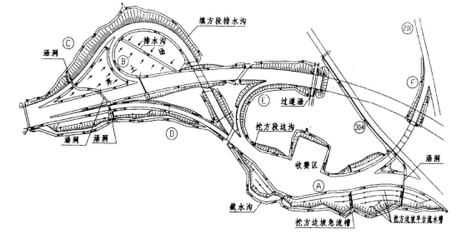
\includegraphics[width=8cm]{排水.png}
            \caption[plain]{立交式排水系统\\图片来源文献\cite{魏明祥2002丹东古城互通式立交的排水设计}}
            \label{fig:my_label}
            \end{figure}
                毗邻地带地表水指路段外自然坡面积水。具体措施是在边坡坡顶外设置截水沟, 沟底建设急流槽, 自然坡面上的流水流入截水沟, 再经急流槽流入边沟或直接经截水沟排出立交区。\upcite{赵阔宇2011浅谈边坡生态防护技术在古城墙保护中绿化的应用}
        \subsubsection{有针对性地加强古城内的绿化工程}
                对于古城墙的维护工作可以采用制草护坡防护的方法,方法如下:在由于年久失修的小部分城墙形成小型的边坡上,种植抗性好外观好且耐虫害的植物,该方法不仅可以对古城墙起到较好的保护作用,并且最大限度减少对于古城原生环境的破坏。
        
                古城内部道路空间有限,我们提议设置街头装饰型绿化,以立体绿化等形式提升街道的绿化覆盖, 改造发展复层群落的种植带式绿化, 从而有效增加绿地面积和绿化率。
                
                在古城外的工业区应设置防护带,工业区与古城间的绿化带宽度不得少于50米,绿化树种应选择对工业有害物质抗性强的乡土树种。\upcite{赵阔宇2011浅谈边坡生态防护技术在古城墙保护中绿化的应用}

                此外,为丰富游客的旅游场景体验,针对绿化植被诸如梨花、杏树等为文化载体,创造性地开设“赏花宴”“踏青节”等颇具历史气息的亲民性活动。
    \subsection{非物质文化遗产的活化利用}
        \subsubsection{开展各种形式的文化活动,增强游客的“获得感”}
        防控疫情不等于一刀切,叫停所有的文化节日活动。坚持“一手撑伞,一手干活”的正确理念,统筹疫情防控常态化与经济社会的复苏发展协调一致,逐渐举办多种类型的文化节日,让非物质文化的展现拥有更大更多的平台,推动文化“活起来”。同时,在继续开展往年举办的中国年、国际摄影大展等的基础上,深入挖掘设立各种纪念活动日与文化交流论坛。 
        \subsubsection{传承传统晋商精神,将情怀为商业文化的核心}
        大力发扬晋商文化,运用到疫情常态化的旅游发展上。将晋商文化中孕育的博大宽厚的胸怀,兼容并蓄的经营气度以及求同存异的经营策略,运用到古城商铺的发展里去。例如创新云旅游的方式,在收到冲击时保持一种情怀大于利益的心态。
    
        开展晋商文化活动,营造特定氛围。商铺可以通过培训员工,在对游客的接待中再现明清晋商精神。政府也可以举办特定的晋商实景剧活动,让游客体验晋商的生活,感受晋商文化,学习票号技术。
    
        \subsubsection{推动“非遗”创造性转化、创新性发展,丰富游客体验}
    
        如果将游客消费点比作一件件商品,而古城的非物质文化遗产就是这些商品精美的包装。推动“非遗 + 住宿”、“非遗 + 创新”、“非遗 + 互联网”等快速皆合,以游客喜闻悦见地方式推广开来,扩大古城文化在时间和空间上的影响力。
    
        “一城两寺”作为一个系统的整体因而不应忽视镇国寺与双林寺的发展。基于文物保护的理念,通过数字化、多元立体化的展示,让民众“零距离”体验平遥雕塑艺术之美,体验“一处触千年”的逼真感。
        \subsubsection{打造特色古城氛围,营造古城历史气息}
            \begin{figure}[H]
                \centering
                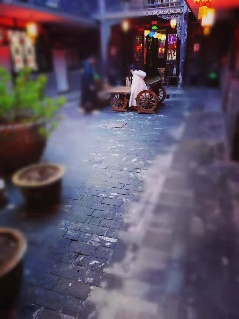
\includegraphics[width=4cm]{汉服.jpeg}
                \caption[plain]{平遥古城内身着古装汉服的游客\\来源:团队于2021年3月摄于平遥某客栈}
                \label{fig:my_label}
            \end{figure}
            不可否认的是,平遥古城最大的特色体现在它完整度极高的“古”上,“古”在城墙建筑,“古”在风土人情。
            
            近年来随着弘扬传统优秀文化意识的不断加强,“古风”文化在青年群体里正带一股来清新的潮流。“着一裳翩翩华服,走一遭古人之路”,年轻群体以这样一种方式打卡人文古迹的现象在古城内非常常见。对于古城内逐渐庞大的这类新群体,政府可予以支持和鼓励,组织兴趣爱好者成立相关协会,同时宣传本地的汉服商铺,推动汉服租用,摄影门店的协同发展,打造“一条龙”服务。
            
            改造传统破旧村落,建设和古城相符的明清建筑风格,同时在古城北部开设更多的非物质遗产商铺,或是连锁本城老字号,以此获取游客注意力,增强旅行体验。
        \subsubsection{创造古城文物衍生品,形成特色古城品牌}
            采取线上推广的形式,设计古城独属的文化形象或者代言人,征集文物的艺术形态,作为古城文化创意产品的品牌标识。同时可以和新媒体公司合作,创造品质高、口碑好的纪录片、综艺片或者影视作品。
            
            同时可以借助丰富的历史文化资源,增强非物质文化遗产品牌建设意识,根据不同年龄段群体,打造适合不同游客层次的“品牌养成计划”。具体来说,针对大部分年轻群体,采用以“文旅结合”为主题,用“寓教于乐,教学相长”的方式,让更多年轻群体参与到非遗品牌建设的完整产业链里。例如开发一款古城历史文化沉浸式体验的游戏;也可增加低年龄段的文创产品供给,比如纸鸢、旋转陀螺,从而改进亲子游群体的游客体验
            \begin{figure}[H]
                \centering
                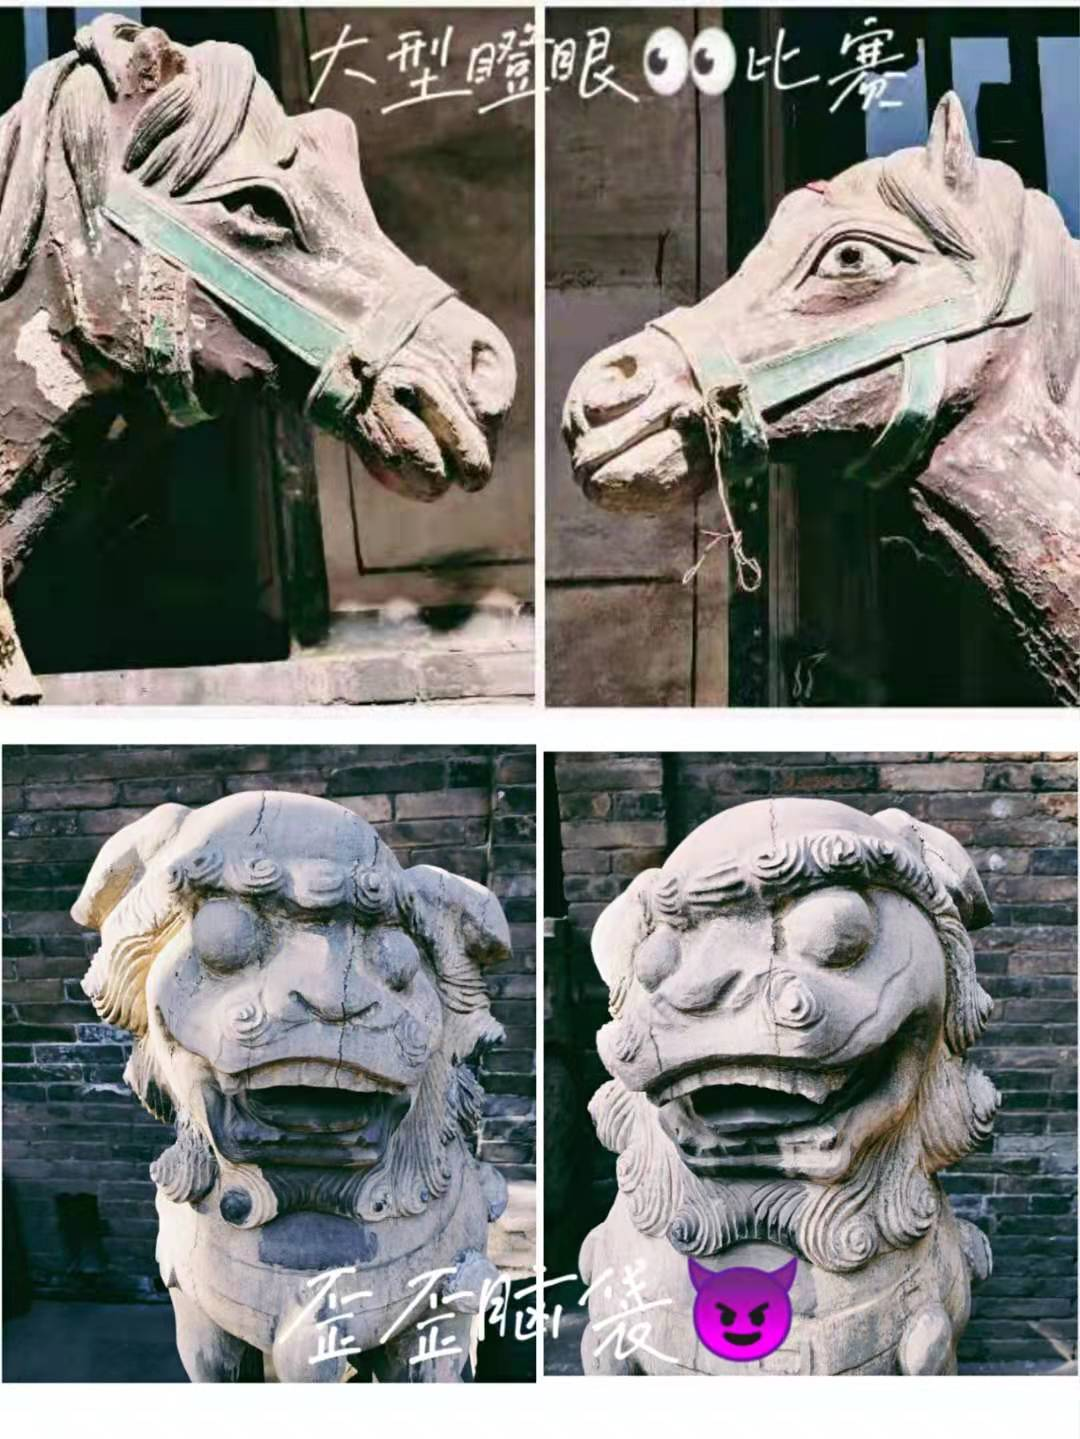
\includegraphics[width=4cm]{表情包.jpg}
                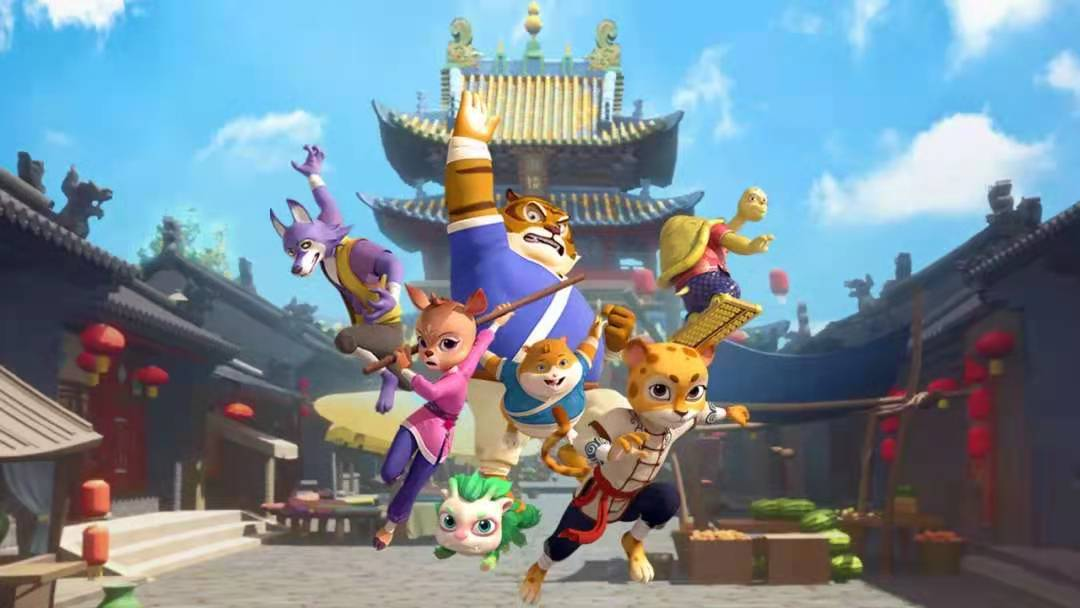
\includegraphics[width=8cm]{古城小镖师.jpg}
                \caption[plain]{带有平遥古城元素的表情包(左)平遥古城的创意动画《古城小镖师》(右)\\资料来源:左图来源于团队自摄加工,右图来源于平遥古城景区官方服务平台公众号}
                \label{fig:my_label}
            \end{figure}
    \subsection{制度设计提升}
    (1).针对劳动群体的不同情况,政府应该安排相关非遗传承人培训技艺技巧。在传承非物质文化遗产同时,通过推广技术的手段来促进非遗特色产品的增进,以“扶智就业”的方式带动经济的发展。例如引进人才,开设传统技艺班,从而建立一套完整统一的保护机制,而后期衍生的产业链既可以传承文化,也可以带动附近居民就业,增加居民经济收入。
    
    (2).形成独特且系统的旅游体系,首先需制定严格的旅游市场管控条例,严厉打击不法经营的现象。其次可通过制定官方标识,将古城内的商铺划分级别,集中管理。同时,设立专职部门监督导游行业。例如解决游客纠纷,只有在官方平台已挂牌的导游方可为其服务。
    
    (3).传承传统文化,每一代都有着不可推卸的责任。借鉴平遥小学义务讲解的事例,可以将平遥县乃至山西省高校列入志愿讲解的行列,以计算志愿讲解时长的方式,由学校组织并鼓励学生前往平遥古城学习讲解。
    
    (4).基于门票方面,可实行“套餐”销售,景区根据不同游客群体的消费心理,可设计多种不同景点结合、门票优惠的方案,增强吸引力。
    
    (5).针对工程项目改造,政府可以借鉴古今中外旅游景点安全事故防范措施,增强对工作人员的考核监督。有计划的推进工程措施,不急功近利,兼顾民生与经济。  
\section{结语}
平遥古城不仅对研究中国历史,借鉴于当今具有不可估量的重要价值,而且作为世界遗产在世界文化宝库中占据着重要地位。在疫情防控期间,平遥古城采取了一系列的措施应对疫情,刺激旅游恢复。其中不乏可圈可点的方面,如政府发令减免商铺租金,疫情防控后期实行免门票的措施等。然而,在如何增强平遥古城对当地经济社会恢复发展的韧性拉动作用方面,尤其是在传承和发扬非物质文化遗产上,挖掘非遗中蕴含的历史蕴意和智慧结晶,创新多种传承途径等,让“平遥古城活起来”,仍存在很大的挖掘空间。而作为非遗的文化载体,对整个平遥古城历史实物的保护,例如古城墙和基础设施的保护,以及文化产品的创新都应纳入考虑范畴之内。疫情之下,衷心希望我们的这些建议能够被关注到并加以采纳,对疫情下的平遥古城开发和可持续发展有所帮助。祝愿平遥古城能够在各个方面做到尽善尽美,成为一处人人流连忘返的旅游胜地,大大提升游客体验感。
    
本文在实地调研的基础上,获取了古城发展情况以及疫情过后的实际情形。伴随着古城旅游业资源的不断挖掘,现实发展的矛盾也接连涌现,疫情的爆发打破了古城保护和发展勉强维持的平衡。政府、游客、商铺之间的利益冲突从另一方面反映了古城保护与利用的侧重。政府也在游客不断的反馈中积极探索新的角度与方向,在保护的前提下合理利用古城资源。但是“大刀阔斧”与“不切实际”的改革现象仍然存在,新的措施在古城相关群体中的推行同样举步维艰。平遥古城吸引力和游客体验的增强仍存在很大的上升空间
    
经过千百年岁月的轮回,平遥古城为后世留下了宝贵的文化遗产。基于游客体验视角的引导,统筹保护古城文物和发展旅游业是目前古城突破困境的出路所在,如何传承并且使其在现代社会推陈出新将会是一个永恒的话题。
    
\nocite{*}
\bibliography{pingyao}
    
\end{document}
